% Options for packages loaded elsewhere
\PassOptionsToPackage{unicode}{hyperref}
\PassOptionsToPackage{hyphens}{url}
%
\documentclass[
]{article}
\usepackage{amsmath,amssymb}
\usepackage{iftex}
\ifPDFTeX
  \usepackage[T1]{fontenc}
  \usepackage[utf8]{inputenc}
  \usepackage{textcomp} % provide euro and other symbols
\else % if luatex or xetex
  \usepackage{unicode-math} % this also loads fontspec
  \defaultfontfeatures{Scale=MatchLowercase}
  \defaultfontfeatures[\rmfamily]{Ligatures=TeX,Scale=1}
\fi
\usepackage{lmodern}
\ifPDFTeX\else
  % xetex/luatex font selection
\fi
% Use upquote if available, for straight quotes in verbatim environments
\IfFileExists{upquote.sty}{\usepackage{upquote}}{}
\IfFileExists{microtype.sty}{% use microtype if available
  \usepackage[]{microtype}
  \UseMicrotypeSet[protrusion]{basicmath} % disable protrusion for tt fonts
}{}
\makeatletter
\@ifundefined{KOMAClassName}{% if non-KOMA class
  \IfFileExists{parskip.sty}{%
    \usepackage{parskip}
  }{% else
    \setlength{\parindent}{0pt}
    \setlength{\parskip}{6pt plus 2pt minus 1pt}}
}{% if KOMA class
  \KOMAoptions{parskip=half}}
\makeatother
\usepackage{xcolor}
\usepackage[margin=1in]{geometry}
\usepackage{color}
\usepackage{fancyvrb}
\newcommand{\VerbBar}{|}
\newcommand{\VERB}{\Verb[commandchars=\\\{\}]}
\DefineVerbatimEnvironment{Highlighting}{Verbatim}{commandchars=\\\{\}}
% Add ',fontsize=\small' for more characters per line
\usepackage{framed}
\definecolor{shadecolor}{RGB}{248,248,248}
\newenvironment{Shaded}{\begin{snugshade}}{\end{snugshade}}
\newcommand{\AlertTok}[1]{\textcolor[rgb]{0.94,0.16,0.16}{#1}}
\newcommand{\AnnotationTok}[1]{\textcolor[rgb]{0.56,0.35,0.01}{\textbf{\textit{#1}}}}
\newcommand{\AttributeTok}[1]{\textcolor[rgb]{0.13,0.29,0.53}{#1}}
\newcommand{\BaseNTok}[1]{\textcolor[rgb]{0.00,0.00,0.81}{#1}}
\newcommand{\BuiltInTok}[1]{#1}
\newcommand{\CharTok}[1]{\textcolor[rgb]{0.31,0.60,0.02}{#1}}
\newcommand{\CommentTok}[1]{\textcolor[rgb]{0.56,0.35,0.01}{\textit{#1}}}
\newcommand{\CommentVarTok}[1]{\textcolor[rgb]{0.56,0.35,0.01}{\textbf{\textit{#1}}}}
\newcommand{\ConstantTok}[1]{\textcolor[rgb]{0.56,0.35,0.01}{#1}}
\newcommand{\ControlFlowTok}[1]{\textcolor[rgb]{0.13,0.29,0.53}{\textbf{#1}}}
\newcommand{\DataTypeTok}[1]{\textcolor[rgb]{0.13,0.29,0.53}{#1}}
\newcommand{\DecValTok}[1]{\textcolor[rgb]{0.00,0.00,0.81}{#1}}
\newcommand{\DocumentationTok}[1]{\textcolor[rgb]{0.56,0.35,0.01}{\textbf{\textit{#1}}}}
\newcommand{\ErrorTok}[1]{\textcolor[rgb]{0.64,0.00,0.00}{\textbf{#1}}}
\newcommand{\ExtensionTok}[1]{#1}
\newcommand{\FloatTok}[1]{\textcolor[rgb]{0.00,0.00,0.81}{#1}}
\newcommand{\FunctionTok}[1]{\textcolor[rgb]{0.13,0.29,0.53}{\textbf{#1}}}
\newcommand{\ImportTok}[1]{#1}
\newcommand{\InformationTok}[1]{\textcolor[rgb]{0.56,0.35,0.01}{\textbf{\textit{#1}}}}
\newcommand{\KeywordTok}[1]{\textcolor[rgb]{0.13,0.29,0.53}{\textbf{#1}}}
\newcommand{\NormalTok}[1]{#1}
\newcommand{\OperatorTok}[1]{\textcolor[rgb]{0.81,0.36,0.00}{\textbf{#1}}}
\newcommand{\OtherTok}[1]{\textcolor[rgb]{0.56,0.35,0.01}{#1}}
\newcommand{\PreprocessorTok}[1]{\textcolor[rgb]{0.56,0.35,0.01}{\textit{#1}}}
\newcommand{\RegionMarkerTok}[1]{#1}
\newcommand{\SpecialCharTok}[1]{\textcolor[rgb]{0.81,0.36,0.00}{\textbf{#1}}}
\newcommand{\SpecialStringTok}[1]{\textcolor[rgb]{0.31,0.60,0.02}{#1}}
\newcommand{\StringTok}[1]{\textcolor[rgb]{0.31,0.60,0.02}{#1}}
\newcommand{\VariableTok}[1]{\textcolor[rgb]{0.00,0.00,0.00}{#1}}
\newcommand{\VerbatimStringTok}[1]{\textcolor[rgb]{0.31,0.60,0.02}{#1}}
\newcommand{\WarningTok}[1]{\textcolor[rgb]{0.56,0.35,0.01}{\textbf{\textit{#1}}}}
\usepackage{graphicx}
\makeatletter
\def\maxwidth{\ifdim\Gin@nat@width>\linewidth\linewidth\else\Gin@nat@width\fi}
\def\maxheight{\ifdim\Gin@nat@height>\textheight\textheight\else\Gin@nat@height\fi}
\makeatother
% Scale images if necessary, so that they will not overflow the page
% margins by default, and it is still possible to overwrite the defaults
% using explicit options in \includegraphics[width, height, ...]{}
\setkeys{Gin}{width=\maxwidth,height=\maxheight,keepaspectratio}
% Set default figure placement to htbp
\makeatletter
\def\fps@figure{htbp}
\makeatother
\setlength{\emergencystretch}{3em} % prevent overfull lines
\providecommand{\tightlist}{%
  \setlength{\itemsep}{0pt}\setlength{\parskip}{0pt}}
\setcounter{secnumdepth}{-\maxdimen} % remove section numbering
\ifLuaTeX
  \usepackage{selnolig}  % disable illegal ligatures
\fi
\IfFileExists{bookmark.sty}{\usepackage{bookmark}}{\usepackage{hyperref}}
\IfFileExists{xurl.sty}{\usepackage{xurl}}{} % add URL line breaks if available
\urlstyle{same}
\hypersetup{
  hidelinks,
  pdfcreator={LaTeX via pandoc}}

\author{}
\date{\vspace{-2.5em}}

\begin{document}

\begin{verbatim}
## 
## 载入程辑包:'dplyr'
\end{verbatim}

\begin{verbatim}
## The following objects are masked from 'package:stats':
## 
##     filter, lag
\end{verbatim}

\begin{verbatim}
## The following objects are masked from 'package:base':
## 
##     intersect, setdiff, setequal, union
\end{verbatim}

\begin{verbatim}
## 
## 载入程辑包:'MASS'
\end{verbatim}

\begin{verbatim}
## The following object is masked from 'package:dplyr':
## 
##     select
\end{verbatim}

\begin{verbatim}
## 载入需要的程辑包:lattice
\end{verbatim}

\begin{verbatim}
## 
## 载入程辑包:'Metrics'
\end{verbatim}

\begin{verbatim}
## The following objects are masked from 'package:caret':
## 
##     precision, recall
\end{verbatim}

\begin{verbatim}
## Warning: 程辑包'pROC'是用R版本4.3.2 来建造的
\end{verbatim}

\begin{verbatim}
## Type 'citation("pROC")' for a citation.
\end{verbatim}

\begin{verbatim}
## 
## 载入程辑包:'pROC'
\end{verbatim}

\begin{verbatim}
## The following object is masked from 'package:Metrics':
## 
##     auc
\end{verbatim}

\begin{verbatim}
## The following objects are masked from 'package:stats':
## 
##     cov, smooth, var
\end{verbatim}

\textbf{Q4.7.10}

This question should be answered using the Weekly data set, which is
part of the ISLR package. This data is similar in nature to the Smarket
data from this chapter's lab, except that it contains 1, 089 weekly
returns for 21 years, from the beginning of 1990 to the end of 2010.

\begin{enumerate}
\def\labelenumi{(\alph{enumi})}
\tightlist
\item
  Produce some numerical and graphical summaries of the Weekly data. Do
  there appear to be any patterns?
\end{enumerate}

\begin{verbatim}
## Rows: 1,089
## Columns: 9
## $ Year      <dbl> 1990, 1990, 1990, 1990, 1990, 1990, 1990, 1990, 1990, 1990, ~
## $ Lag1      <dbl> 0.816, -0.270, -2.576, 3.514, 0.712, 1.178, -1.372, 0.807, 0~
## $ Lag2      <dbl> 1.572, 0.816, -0.270, -2.576, 3.514, 0.712, 1.178, -1.372, 0~
## $ Lag3      <dbl> -3.936, 1.572, 0.816, -0.270, -2.576, 3.514, 0.712, 1.178, -~
## $ Lag4      <dbl> -0.229, -3.936, 1.572, 0.816, -0.270, -2.576, 3.514, 0.712, ~
## $ Lag5      <dbl> -3.484, -0.229, -3.936, 1.572, 0.816, -0.270, -2.576, 3.514,~
## $ Volume    <dbl> 0.1549760, 0.1485740, 0.1598375, 0.1616300, 0.1537280, 0.154~
## $ Today     <dbl> -0.270, -2.576, 3.514, 0.712, 1.178, -1.372, 0.807, 0.041, 1~
## $ Direction <fct> Down, Down, Up, Up, Up, Down, Up, Up, Up, Down, Down, Up, Up~
\end{verbatim}

\begin{Shaded}
\begin{Highlighting}[]
\FunctionTok{par}\NormalTok{(}\AttributeTok{family =} \StringTok{"mono"}\NormalTok{)}
\FunctionTok{pairs}\NormalTok{(Weekly[, }\SpecialCharTok{{-}}\DecValTok{9}\NormalTok{])}
\end{Highlighting}
\end{Shaded}

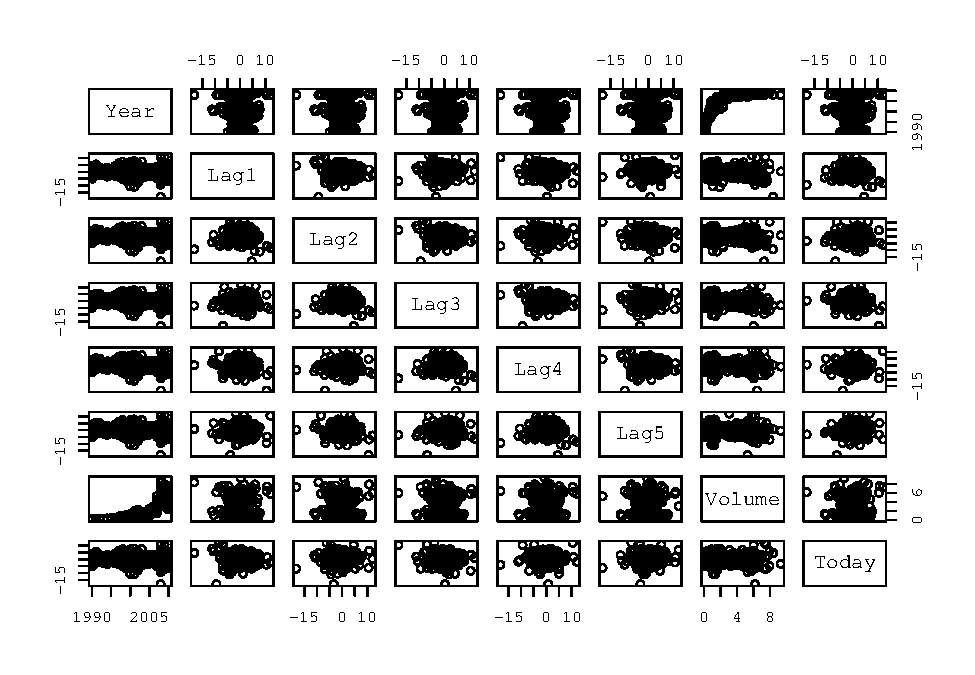
\includegraphics{ISLR4.7.10_files/figure-latex/unnamed-chunk-3-1.pdf}

\begin{Shaded}
\begin{Highlighting}[]
\FunctionTok{par}\NormalTok{(}\AttributeTok{family =} \StringTok{"mono"}\NormalTok{)}
\FunctionTok{plot}\NormalTok{(Weekly}\SpecialCharTok{$}\NormalTok{Volume, }\AttributeTok{main =} \StringTok{"Volume vs. Time"}\NormalTok{, }\AttributeTok{xlab =} \StringTok{"Time (Trading day)"}\NormalTok{, }\AttributeTok{ylab =} \StringTok{"Volume (Billion)"}\NormalTok{)}
\end{Highlighting}
\end{Shaded}

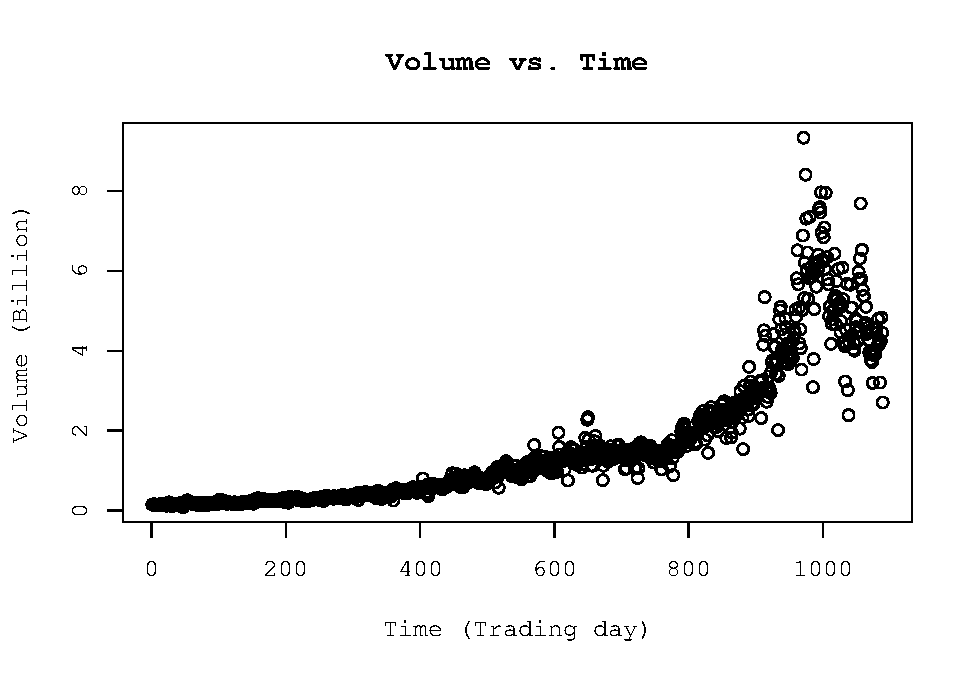
\includegraphics{ISLR4.7.10_files/figure-latex/unnamed-chunk-4-1.pdf}

\begin{enumerate}
\def\labelenumi{(\alph{enumi})}
\setcounter{enumi}{1}
\tightlist
\item
  Use the full data set to perform a logistic regression with Direction
  as the response and the five lag variables plus Volume as predictors.
  Use the summary function to print the results. Do any of the
  predictors appear to be statistically significant? If so, which ones?
\end{enumerate}

The predictor Lag2 appears to be statistically significant.

\begin{verbatim}
## 
## Call:
## glm(formula = Direction ~ Lag1 + Lag2 + Lag3 + Lag4 + Lag5 + 
##     Volume, family = binomial(), data = Weekly)
## 
## Coefficients:
##             Estimate Std. Error z value Pr(>|z|)   
## (Intercept)  0.26686    0.08593   3.106   0.0019 **
## Lag1        -0.04127    0.02641  -1.563   0.1181   
## Lag2         0.05844    0.02686   2.175   0.0296 * 
## Lag3        -0.01606    0.02666  -0.602   0.5469   
## Lag4        -0.02779    0.02646  -1.050   0.2937   
## Lag5        -0.01447    0.02638  -0.549   0.5833   
## Volume      -0.02274    0.03690  -0.616   0.5377   
## ---
## Signif. codes:  0 '***' 0.001 '**' 0.01 '*' 0.05 '.' 0.1 ' ' 1
## 
## (Dispersion parameter for binomial family taken to be 1)
## 
##     Null deviance: 1496.2  on 1088  degrees of freedom
## Residual deviance: 1486.4  on 1082  degrees of freedom
## AIC: 1500.4
## 
## Number of Fisher Scoring iterations: 4
\end{verbatim}

\begin{enumerate}
\def\labelenumi{(\alph{enumi})}
\setcounter{enumi}{2}
\tightlist
\item
  Compute the confusion matrix and overall fraction of correct
  predictions. Explain what the confusion matrix is telling you about
  the types of mistakes made by logistic regression.
\end{enumerate}

The confusion matrix shows the performance of a logistic regression
model. In this case, it tells us that the model correctly predicted 54
instances of ``Down'' and 557 instances of ``Up.'' However, it made 430
false negatives (predicted ``Up'' when it was ``Down'') and 48 false
positives (predicted ``Down'' when it was ``Up'').

\begin{Shaded}
\begin{Highlighting}[]
\NormalTok{p }\OtherTok{=} \FunctionTok{predict}\NormalTok{(log\_res, }\AttributeTok{type =} \StringTok{"response"}\NormalTok{)}
\NormalTok{predicted\_direction }\OtherTok{=} \FunctionTok{ifelse}\NormalTok{(p }\SpecialCharTok{\textgreater{}} \FloatTok{0.5}\NormalTok{, }\StringTok{"Up"}\NormalTok{, }\StringTok{"Down"}\NormalTok{)}
\NormalTok{confusion\_matrix }\OtherTok{=} \FunctionTok{table}\NormalTok{(}\AttributeTok{Actual =}\NormalTok{ Weekly}\SpecialCharTok{$}\NormalTok{Direction, }\AttributeTok{Predicted =}\NormalTok{ predicted\_direction)}
\NormalTok{confusion\_matrix}
\end{Highlighting}
\end{Shaded}

\begin{verbatim}
##       Predicted
## Actual Down  Up
##   Down   54 430
##   Up     48 557
\end{verbatim}

\begin{Shaded}
\begin{Highlighting}[]
\NormalTok{accuracy }\OtherTok{=} \FunctionTok{sum}\NormalTok{(}\FunctionTok{diag}\NormalTok{(confusion\_matrix)) }\SpecialCharTok{/} \FunctionTok{sum}\NormalTok{(confusion\_matrix)}
\FunctionTok{cat}\NormalTok{(}\StringTok{"Overall Fraction of Correct Predictions:"}\NormalTok{, accuracy, }\StringTok{"}\SpecialCharTok{\textbackslash{}n}\StringTok{"}\NormalTok{)}
\end{Highlighting}
\end{Shaded}

\begin{verbatim}
## Overall Fraction of Correct Predictions: 0.5610652
\end{verbatim}

\begin{enumerate}
\def\labelenumi{(\alph{enumi})}
\setcounter{enumi}{3}
\tightlist
\item
  Now fit the logistic regression model using a training data period
  from 1990 to 2008, with Lag2 as the only predictor. Compute the
  confusion matrix and the overall fraction of correct predictions for
  the held out data (that is, the data from 2009 and 2010).
\end{enumerate}

\begin{Shaded}
\begin{Highlighting}[]
\NormalTok{training\_data }\OtherTok{=}\NormalTok{ Weekly[Weekly}\SpecialCharTok{$}\NormalTok{Year }\SpecialCharTok{\textless{}=} \DecValTok{2008}\NormalTok{,]}
\NormalTok{test\_data }\OtherTok{=}\NormalTok{ Weekly[Weekly}\SpecialCharTok{$}\NormalTok{Year }\SpecialCharTok{\textgreater{}} \DecValTok{2008}\NormalTok{,]}
\NormalTok{model }\OtherTok{=} \FunctionTok{glm}\NormalTok{(Direction }\SpecialCharTok{\textasciitilde{}}\NormalTok{ Lag2, }\AttributeTok{data =}\NormalTok{ training\_data, }\AttributeTok{family =}\NormalTok{ binomial)}
\NormalTok{predicted\_probs }\OtherTok{=} \FunctionTok{predict}\NormalTok{(model, }\AttributeTok{newdata =}\NormalTok{ test\_data, }\AttributeTok{type =} \StringTok{"response"}\NormalTok{)}
\NormalTok{predicted\_direction }\OtherTok{=} \FunctionTok{ifelse}\NormalTok{(predicted\_probs }\SpecialCharTok{\textgreater{}} \FloatTok{0.5}\NormalTok{, }\StringTok{"Up"}\NormalTok{, }\StringTok{"Down"}\NormalTok{)}

\NormalTok{confusion\_matrix }\OtherTok{=} \FunctionTok{table}\NormalTok{(}\AttributeTok{Actual =}\NormalTok{ test\_data}\SpecialCharTok{$}\NormalTok{Direction, }\AttributeTok{Predicted =}\NormalTok{ predicted\_direction)}
\NormalTok{confusion\_matrix}
\end{Highlighting}
\end{Shaded}

\begin{verbatim}
##       Predicted
## Actual Down Up
##   Down    9 34
##   Up      5 56
\end{verbatim}

\begin{Shaded}
\begin{Highlighting}[]
\NormalTok{accuracy }\OtherTok{\textless{}{-}} \FunctionTok{sum}\NormalTok{(}\FunctionTok{diag}\NormalTok{(confusion\_matrix)) }\SpecialCharTok{/} \FunctionTok{sum}\NormalTok{(confusion\_matrix)}

\FunctionTok{cat}\NormalTok{(}\StringTok{"Overall Fraction of Correct Predictions:"}\NormalTok{, accuracy, }\StringTok{"}\SpecialCharTok{\textbackslash{}n}\StringTok{"}\NormalTok{)}
\end{Highlighting}
\end{Shaded}

\begin{verbatim}
## Overall Fraction of Correct Predictions: 0.625
\end{verbatim}

\begin{enumerate}
\def\labelenumi{(\alph{enumi})}
\setcounter{enumi}{4}
\tightlist
\item
  Repeat (d) using LDA.
\end{enumerate}

\begin{Shaded}
\begin{Highlighting}[]
\NormalTok{lda\_model }\OtherTok{=} \FunctionTok{lda}\NormalTok{(Direction }\SpecialCharTok{\textasciitilde{}}\NormalTok{ Lag2, }\AttributeTok{data =}\NormalTok{ training\_data)}
\NormalTok{predicted\_probs }\OtherTok{=} \FunctionTok{predict}\NormalTok{(lda\_model, }\AttributeTok{newdata =}\NormalTok{ test\_data, }\AttributeTok{type =} \StringTok{"response"}\NormalTok{)}
\NormalTok{predicted\_direction }\OtherTok{=} \FunctionTok{predict}\NormalTok{(lda\_model, }\AttributeTok{newdata =}\NormalTok{ test\_data)}\SpecialCharTok{$}\NormalTok{class}

\NormalTok{confusion\_matrix }\OtherTok{=} \FunctionTok{table}\NormalTok{(}\AttributeTok{Actual =}\NormalTok{ test\_data}\SpecialCharTok{$}\NormalTok{Direction, }\AttributeTok{Predicted =}\NormalTok{ predicted\_direction)}
\NormalTok{confusion\_matrix}
\end{Highlighting}
\end{Shaded}

\begin{verbatim}
##       Predicted
## Actual Down Up
##   Down    9 34
##   Up      5 56
\end{verbatim}

\begin{Shaded}
\begin{Highlighting}[]
\NormalTok{accuracy }\OtherTok{=} \FunctionTok{sum}\NormalTok{(}\FunctionTok{diag}\NormalTok{(confusion\_matrix)) }\SpecialCharTok{/} \FunctionTok{sum}\NormalTok{(confusion\_matrix)}

\FunctionTok{cat}\NormalTok{(}\StringTok{"Overall Fraction of Correct Predictions:"}\NormalTok{, accuracy, }\StringTok{"}\SpecialCharTok{\textbackslash{}n}\StringTok{"}\NormalTok{)}
\end{Highlighting}
\end{Shaded}

\begin{verbatim}
## Overall Fraction of Correct Predictions: 0.625
\end{verbatim}

\begin{enumerate}
\def\labelenumi{(\alph{enumi})}
\setcounter{enumi}{5}
\tightlist
\item
  Repeat (d) using QDA.
\end{enumerate}

\begin{Shaded}
\begin{Highlighting}[]
\NormalTok{qda\_model }\OtherTok{=} \FunctionTok{qda}\NormalTok{(Direction }\SpecialCharTok{\textasciitilde{}}\NormalTok{ Lag2, }\AttributeTok{data =}\NormalTok{ training\_data)}
\NormalTok{predicted\_probs }\OtherTok{=} \FunctionTok{predict}\NormalTok{(qda\_model, }\AttributeTok{newdata =}\NormalTok{ test\_data, }\AttributeTok{type =} \StringTok{"response"}\NormalTok{)}
\NormalTok{predicted\_direction }\OtherTok{=} \FunctionTok{predict}\NormalTok{(qda\_model, }\AttributeTok{newdata =}\NormalTok{ test\_data)}\SpecialCharTok{$}\NormalTok{class}

\NormalTok{confusion\_matrix }\OtherTok{=} \FunctionTok{table}\NormalTok{(}\AttributeTok{Actual =}\NormalTok{ test\_data}\SpecialCharTok{$}\NormalTok{Direction, }\AttributeTok{Predicted =}\NormalTok{ predicted\_direction)}
\NormalTok{confusion\_matrix}
\end{Highlighting}
\end{Shaded}

\begin{verbatim}
##       Predicted
## Actual Down Up
##   Down    0 43
##   Up      0 61
\end{verbatim}

\begin{Shaded}
\begin{Highlighting}[]
\NormalTok{accuracy }\OtherTok{=} \FunctionTok{sum}\NormalTok{(}\FunctionTok{diag}\NormalTok{(confusion\_matrix)) }\SpecialCharTok{/} \FunctionTok{sum}\NormalTok{(confusion\_matrix)}

\FunctionTok{cat}\NormalTok{(}\StringTok{"Overall Fraction of Correct Predictions:"}\NormalTok{, accuracy, }\StringTok{"}\SpecialCharTok{\textbackslash{}n}\StringTok{"}\NormalTok{)}
\end{Highlighting}
\end{Shaded}

\begin{verbatim}
## Overall Fraction of Correct Predictions: 0.5865385
\end{verbatim}

\begin{enumerate}
\def\labelenumi{(\alph{enumi})}
\setcounter{enumi}{6}
\tightlist
\item
  Repeat (d) using KNN with K = 1.
\end{enumerate}

\begin{Shaded}
\begin{Highlighting}[]
\NormalTok{knn\_model }\OtherTok{=} \FunctionTok{knn}\NormalTok{(}\AttributeTok{train =} \FunctionTok{cbind}\NormalTok{(training\_data}\SpecialCharTok{$}\NormalTok{Lag2), }\AttributeTok{test =} \FunctionTok{cbind}\NormalTok{(test\_data}\SpecialCharTok{$}\NormalTok{Lag2), }\AttributeTok{cl =}\NormalTok{ training\_data}\SpecialCharTok{$}\NormalTok{Direction, }\AttributeTok{k =} \DecValTok{1}\NormalTok{)}
\NormalTok{confusion\_matrix }\OtherTok{=} \FunctionTok{table}\NormalTok{(}\AttributeTok{Actual =}\NormalTok{ test\_data}\SpecialCharTok{$}\NormalTok{Direction, }\AttributeTok{Predicted =}\NormalTok{ knn\_model)}
\NormalTok{confusion\_matrix}
\end{Highlighting}
\end{Shaded}

\begin{verbatim}
##       Predicted
## Actual Down Up
##   Down   21 22
##   Up     30 31
\end{verbatim}

\begin{Shaded}
\begin{Highlighting}[]
\NormalTok{accuracy }\OtherTok{=} \FunctionTok{sum}\NormalTok{(}\FunctionTok{diag}\NormalTok{(confusion\_matrix)) }\SpecialCharTok{/} \FunctionTok{sum}\NormalTok{(confusion\_matrix)}

\FunctionTok{cat}\NormalTok{(}\StringTok{"Overall Fraction of Correct Predictions:"}\NormalTok{, accuracy, }\StringTok{"}\SpecialCharTok{\textbackslash{}n}\StringTok{"}\NormalTok{)}
\end{Highlighting}
\end{Shaded}

\begin{verbatim}
## Overall Fraction of Correct Predictions: 0.5
\end{verbatim}

\begin{enumerate}
\def\labelenumi{(\alph{enumi})}
\setcounter{enumi}{7}
\tightlist
\item
  Which of these methods appears to provide the best results on this
  data?
\end{enumerate}

By simply comparing accuracies, LDA performs the best.

\begin{enumerate}
\def\labelenumi{(\roman{enumi})}
\tightlist
\item
  Experiment with different combinations of predictors, including
  possible transformations and interactions, for each of the methods.
  Report the variables, method, and associated confusion matrix that
  appears to provide the best results on the held out data. Note that
  you should also experiment with values for K in the KNN classifier.
\end{enumerate}

7 different combinations are tested as follows, and QDA with Multiple
Variable Interactions performs the best, with accuracy of 64.4\%.

\begin{Shaded}
\begin{Highlighting}[]
\CommentTok{\# KNN with K = 3}
\NormalTok{knn\_model }\OtherTok{=} \FunctionTok{knn}\NormalTok{(}\AttributeTok{train =} \FunctionTok{cbind}\NormalTok{(training\_data}\SpecialCharTok{$}\NormalTok{Lag2), }\AttributeTok{test =} \FunctionTok{cbind}\NormalTok{(test\_data}\SpecialCharTok{$}\NormalTok{Lag2), }\AttributeTok{cl =}\NormalTok{ training\_data}\SpecialCharTok{$}\NormalTok{Direction, }\AttributeTok{k =} \DecValTok{3}\NormalTok{)}
\NormalTok{confusion\_matrix }\OtherTok{=} \FunctionTok{table}\NormalTok{(}\AttributeTok{Actual =}\NormalTok{ test\_data}\SpecialCharTok{$}\NormalTok{Direction, }\AttributeTok{Predicted =}\NormalTok{ knn\_model)}
\NormalTok{accuracy }\OtherTok{=} \FunctionTok{sum}\NormalTok{(}\FunctionTok{diag}\NormalTok{(confusion\_matrix)) }\SpecialCharTok{/} \FunctionTok{sum}\NormalTok{(confusion\_matrix)}
\FunctionTok{cat}\NormalTok{(}\StringTok{"KNN with K = 3:}\SpecialCharTok{\textbackslash{}n}\StringTok{"}\NormalTok{)}
\end{Highlighting}
\end{Shaded}

\begin{verbatim}
## KNN with K = 3:
\end{verbatim}

\begin{Shaded}
\begin{Highlighting}[]
\FunctionTok{cat}\NormalTok{(}\StringTok{"Overall Fraction of Correct Predictions:"}\NormalTok{, accuracy, }\StringTok{"}\SpecialCharTok{\textbackslash{}n}\StringTok{"}\NormalTok{)}
\end{Highlighting}
\end{Shaded}

\begin{verbatim}
## Overall Fraction of Correct Predictions: 0.5480769
\end{verbatim}

\begin{Shaded}
\begin{Highlighting}[]
\FunctionTok{print}\NormalTok{(confusion\_matrix)}
\end{Highlighting}
\end{Shaded}

\begin{verbatim}
##       Predicted
## Actual Down Up
##   Down   15 28
##   Up     19 42
\end{verbatim}

\begin{Shaded}
\begin{Highlighting}[]
\FunctionTok{cat}\NormalTok{(}\StringTok{"}\SpecialCharTok{\textbackslash{}n}\StringTok{"}\NormalTok{)}
\end{Highlighting}
\end{Shaded}

\begin{Shaded}
\begin{Highlighting}[]
\CommentTok{\# KNN with K = 5}
\NormalTok{knn\_model }\OtherTok{=} \FunctionTok{knn}\NormalTok{(}\AttributeTok{train =} \FunctionTok{cbind}\NormalTok{(training\_data}\SpecialCharTok{$}\NormalTok{Lag2), }\AttributeTok{test =} \FunctionTok{cbind}\NormalTok{(test\_data}\SpecialCharTok{$}\NormalTok{Lag2), }\AttributeTok{cl =}\NormalTok{ training\_data}\SpecialCharTok{$}\NormalTok{Direction, }\AttributeTok{k =} \DecValTok{5}\NormalTok{)}
\NormalTok{confusion\_matrix }\OtherTok{=} \FunctionTok{table}\NormalTok{(}\AttributeTok{Actual =}\NormalTok{ test\_data}\SpecialCharTok{$}\NormalTok{Direction, }\AttributeTok{Predicted =}\NormalTok{ knn\_model)}
\NormalTok{accuracy }\OtherTok{=} \FunctionTok{sum}\NormalTok{(}\FunctionTok{diag}\NormalTok{(confusion\_matrix)) }\SpecialCharTok{/} \FunctionTok{sum}\NormalTok{(confusion\_matrix)}
\FunctionTok{cat}\NormalTok{(}\StringTok{"KNN with K = 5:}\SpecialCharTok{\textbackslash{}n}\StringTok{"}\NormalTok{)}
\end{Highlighting}
\end{Shaded}

\begin{verbatim}
## KNN with K = 5:
\end{verbatim}

\begin{Shaded}
\begin{Highlighting}[]
\FunctionTok{cat}\NormalTok{(}\StringTok{"Overall Fraction of Correct Predictions:"}\NormalTok{, accuracy, }\StringTok{"}\SpecialCharTok{\textbackslash{}n}\StringTok{"}\NormalTok{)}
\end{Highlighting}
\end{Shaded}

\begin{verbatim}
## Overall Fraction of Correct Predictions: 0.5384615
\end{verbatim}

\begin{Shaded}
\begin{Highlighting}[]
\FunctionTok{print}\NormalTok{(confusion\_matrix)}
\end{Highlighting}
\end{Shaded}

\begin{verbatim}
##       Predicted
## Actual Down Up
##   Down   16 27
##   Up     21 40
\end{verbatim}

\begin{Shaded}
\begin{Highlighting}[]
\FunctionTok{cat}\NormalTok{(}\StringTok{"}\SpecialCharTok{\textbackslash{}n}\StringTok{"}\NormalTok{)}
\end{Highlighting}
\end{Shaded}

\begin{Shaded}
\begin{Highlighting}[]
\CommentTok{\# KNN with K = 10}
\NormalTok{knn\_model }\OtherTok{=} \FunctionTok{knn}\NormalTok{(}\AttributeTok{train =} \FunctionTok{cbind}\NormalTok{(training\_data}\SpecialCharTok{$}\NormalTok{Lag2), }\AttributeTok{test =} \FunctionTok{cbind}\NormalTok{(test\_data}\SpecialCharTok{$}\NormalTok{Lag2), }\AttributeTok{cl =}\NormalTok{ training\_data}\SpecialCharTok{$}\NormalTok{Direction, }\AttributeTok{k =} \DecValTok{10}\NormalTok{)}
\NormalTok{confusion\_matrix }\OtherTok{=} \FunctionTok{table}\NormalTok{(}\AttributeTok{Actual =}\NormalTok{ test\_data}\SpecialCharTok{$}\NormalTok{Direction, }\AttributeTok{Predicted =}\NormalTok{ knn\_model)}
\NormalTok{accuracy }\OtherTok{=} \FunctionTok{sum}\NormalTok{(}\FunctionTok{diag}\NormalTok{(confusion\_matrix)) }\SpecialCharTok{/} \FunctionTok{sum}\NormalTok{(confusion\_matrix)}
\FunctionTok{cat}\NormalTok{(}\StringTok{"KNN with K = 10:}\SpecialCharTok{\textbackslash{}n}\StringTok{"}\NormalTok{)}
\end{Highlighting}
\end{Shaded}

\begin{verbatim}
## KNN with K = 10:
\end{verbatim}

\begin{Shaded}
\begin{Highlighting}[]
\FunctionTok{cat}\NormalTok{(}\StringTok{"Overall Fraction of Correct Predictions:"}\NormalTok{, accuracy, }\StringTok{"}\SpecialCharTok{\textbackslash{}n}\StringTok{"}\NormalTok{)}
\end{Highlighting}
\end{Shaded}

\begin{verbatim}
## Overall Fraction of Correct Predictions: 0.5576923
\end{verbatim}

\begin{Shaded}
\begin{Highlighting}[]
\FunctionTok{print}\NormalTok{(confusion\_matrix)}
\end{Highlighting}
\end{Shaded}

\begin{verbatim}
##       Predicted
## Actual Down Up
##   Down   16 27
##   Up     19 42
\end{verbatim}

\begin{Shaded}
\begin{Highlighting}[]
\FunctionTok{cat}\NormalTok{(}\StringTok{"}\SpecialCharTok{\textbackslash{}n}\StringTok{"}\NormalTok{)}
\end{Highlighting}
\end{Shaded}

\begin{Shaded}
\begin{Highlighting}[]
\CommentTok{\# LDA with Multiple Variables}
\NormalTok{lda\_model }\OtherTok{=} \FunctionTok{lda}\NormalTok{(Direction }\SpecialCharTok{\textasciitilde{}}\NormalTok{ Lag1 }\SpecialCharTok{+}\NormalTok{ Lag2 }\SpecialCharTok{+}\NormalTok{ Lag3 }\SpecialCharTok{+}\NormalTok{ Lag4 }\SpecialCharTok{+}\NormalTok{ Lag5, }\AttributeTok{data =}\NormalTok{ training\_data)}
\NormalTok{predicted\_probs }\OtherTok{=} \FunctionTok{predict}\NormalTok{(lda\_model, }\AttributeTok{newdata =}\NormalTok{ test\_data, }\AttributeTok{type =} \StringTok{"response"}\NormalTok{)}
\NormalTok{predicted\_direction }\OtherTok{=} \FunctionTok{predict}\NormalTok{(lda\_model, }\AttributeTok{newdata =}\NormalTok{ test\_data)}\SpecialCharTok{$}\NormalTok{class}
\NormalTok{confusion\_matrix }\OtherTok{=} \FunctionTok{table}\NormalTok{(}\AttributeTok{Actual =}\NormalTok{ test\_data}\SpecialCharTok{$}\NormalTok{Direction, }\AttributeTok{Predicted =}\NormalTok{ predicted\_direction)}
\FunctionTok{cat}\NormalTok{(}\StringTok{"LDA with Multiple Variables}\SpecialCharTok{\textbackslash{}n}\StringTok{"}\NormalTok{)}
\end{Highlighting}
\end{Shaded}

\begin{verbatim}
## LDA with Multiple Variables
\end{verbatim}

\begin{Shaded}
\begin{Highlighting}[]
\NormalTok{accuracy }\OtherTok{=} \FunctionTok{sum}\NormalTok{(}\FunctionTok{diag}\NormalTok{(confusion\_matrix)) }\SpecialCharTok{/} \FunctionTok{sum}\NormalTok{(confusion\_matrix)}
\FunctionTok{cat}\NormalTok{(}\StringTok{"Overall Fraction of Correct Predictions:"}\NormalTok{, accuracy, }\StringTok{"}\SpecialCharTok{\textbackslash{}n}\StringTok{"}\NormalTok{)}
\end{Highlighting}
\end{Shaded}

\begin{verbatim}
## Overall Fraction of Correct Predictions: 0.5480769
\end{verbatim}

\begin{Shaded}
\begin{Highlighting}[]
\FunctionTok{print}\NormalTok{(confusion\_matrix)}
\end{Highlighting}
\end{Shaded}

\begin{verbatim}
##       Predicted
## Actual Down Up
##   Down    9 34
##   Up     13 48
\end{verbatim}

\begin{Shaded}
\begin{Highlighting}[]
\FunctionTok{cat}\NormalTok{(}\StringTok{"}\SpecialCharTok{\textbackslash{}n}\StringTok{"}\NormalTok{)}
\end{Highlighting}
\end{Shaded}

\begin{Shaded}
\begin{Highlighting}[]
\CommentTok{\# LDA with Multiple Variable Interactions}
\NormalTok{lda\_model }\OtherTok{=} \FunctionTok{lda}\NormalTok{(Direction }\SpecialCharTok{\textasciitilde{}}\NormalTok{ (Lag1 }\SpecialCharTok{+}\NormalTok{ Lag2 }\SpecialCharTok{+}\NormalTok{ Lag3 }\SpecialCharTok{+}\NormalTok{ Lag4 }\SpecialCharTok{+}\NormalTok{ Lag5)}\SpecialCharTok{\^{}}\DecValTok{2}\NormalTok{, }\AttributeTok{data =}\NormalTok{ training\_data)}
\NormalTok{predicted\_probs }\OtherTok{=} \FunctionTok{predict}\NormalTok{(lda\_model, }\AttributeTok{newdata =}\NormalTok{ test\_data, }\AttributeTok{type =} \StringTok{"response"}\NormalTok{)}
\NormalTok{predicted\_direction }\OtherTok{=} \FunctionTok{predict}\NormalTok{(lda\_model, }\AttributeTok{newdata =}\NormalTok{ test\_data)}\SpecialCharTok{$}\NormalTok{class}
\NormalTok{confusion\_matrix }\OtherTok{=} \FunctionTok{table}\NormalTok{(}\AttributeTok{Actual =}\NormalTok{ test\_data}\SpecialCharTok{$}\NormalTok{Direction, }\AttributeTok{Predicted =}\NormalTok{ predicted\_direction)}
\FunctionTok{cat}\NormalTok{(}\StringTok{"LDA with Multiple Variable Interactions}\SpecialCharTok{\textbackslash{}n}\StringTok{"}\NormalTok{)}
\end{Highlighting}
\end{Shaded}

\begin{verbatim}
## LDA with Multiple Variable Interactions
\end{verbatim}

\begin{Shaded}
\begin{Highlighting}[]
\NormalTok{accuracy }\OtherTok{=} \FunctionTok{sum}\NormalTok{(}\FunctionTok{diag}\NormalTok{(confusion\_matrix)) }\SpecialCharTok{/} \FunctionTok{sum}\NormalTok{(confusion\_matrix)}
\FunctionTok{cat}\NormalTok{(}\StringTok{"Overall Fraction of Correct Predictions:"}\NormalTok{, accuracy, }\StringTok{"}\SpecialCharTok{\textbackslash{}n}\StringTok{"}\NormalTok{)}
\end{Highlighting}
\end{Shaded}

\begin{verbatim}
## Overall Fraction of Correct Predictions: 0.5288462
\end{verbatim}

\begin{Shaded}
\begin{Highlighting}[]
\FunctionTok{print}\NormalTok{(confusion\_matrix)}
\end{Highlighting}
\end{Shaded}

\begin{verbatim}
##       Predicted
## Actual Down Up
##   Down   10 33
##   Up     16 45
\end{verbatim}

\begin{Shaded}
\begin{Highlighting}[]
\FunctionTok{cat}\NormalTok{(}\StringTok{"}\SpecialCharTok{\textbackslash{}n}\StringTok{"}\NormalTok{)}
\end{Highlighting}
\end{Shaded}

\begin{Shaded}
\begin{Highlighting}[]
\CommentTok{\# QDA with Multiple Variables}
\NormalTok{qda\_model }\OtherTok{=} \FunctionTok{qda}\NormalTok{(Direction }\SpecialCharTok{\textasciitilde{}}\NormalTok{ Lag1 }\SpecialCharTok{+}\NormalTok{ Lag2 }\SpecialCharTok{+}\NormalTok{ Lag3 }\SpecialCharTok{+}\NormalTok{ Lag4 }\SpecialCharTok{+}\NormalTok{ Lag5, }\AttributeTok{data =}\NormalTok{ training\_data)}
\NormalTok{predicted\_probs }\OtherTok{=} \FunctionTok{predict}\NormalTok{(qda\_model, }\AttributeTok{newdata =}\NormalTok{ test\_data, }\AttributeTok{type =} \StringTok{"response"}\NormalTok{)}
\NormalTok{predicted\_direction }\OtherTok{=} \FunctionTok{predict}\NormalTok{(qda\_model, }\AttributeTok{newdata =}\NormalTok{ test\_data)}\SpecialCharTok{$}\NormalTok{class}
\NormalTok{confusion\_matrix }\OtherTok{=} \FunctionTok{table}\NormalTok{(}\AttributeTok{Actual =}\NormalTok{ test\_data}\SpecialCharTok{$}\NormalTok{Direction, }\AttributeTok{Predicted =}\NormalTok{ predicted\_direction)}
\FunctionTok{cat}\NormalTok{(}\StringTok{"QDA with Multiple Variables}\SpecialCharTok{\textbackslash{}n}\StringTok{"}\NormalTok{)}
\end{Highlighting}
\end{Shaded}

\begin{verbatim}
## QDA with Multiple Variables
\end{verbatim}

\begin{Shaded}
\begin{Highlighting}[]
\NormalTok{accuracy }\OtherTok{=} \FunctionTok{sum}\NormalTok{(}\FunctionTok{diag}\NormalTok{(confusion\_matrix)) }\SpecialCharTok{/} \FunctionTok{sum}\NormalTok{(confusion\_matrix)}
\FunctionTok{cat}\NormalTok{(}\StringTok{"Overall Fraction of Correct Predictions:"}\NormalTok{, accuracy, }\StringTok{"}\SpecialCharTok{\textbackslash{}n}\StringTok{"}\NormalTok{)}
\end{Highlighting}
\end{Shaded}

\begin{verbatim}
## Overall Fraction of Correct Predictions: 0.4615385
\end{verbatim}

\begin{Shaded}
\begin{Highlighting}[]
\FunctionTok{print}\NormalTok{(confusion\_matrix)}
\end{Highlighting}
\end{Shaded}

\begin{verbatim}
##       Predicted
## Actual Down Up
##   Down   10 33
##   Up     23 38
\end{verbatim}

\begin{Shaded}
\begin{Highlighting}[]
\FunctionTok{cat}\NormalTok{(}\StringTok{"}\SpecialCharTok{\textbackslash{}n}\StringTok{"}\NormalTok{)}
\end{Highlighting}
\end{Shaded}

\begin{Shaded}
\begin{Highlighting}[]
\CommentTok{\# QDA with Multiple Variable Interactions}
\NormalTok{qda\_model }\OtherTok{=} \FunctionTok{qda}\NormalTok{(Direction }\SpecialCharTok{\textasciitilde{}}\NormalTok{ (Lag1 }\SpecialCharTok{+}\NormalTok{ Lag2 }\SpecialCharTok{+}\NormalTok{ Lag3 }\SpecialCharTok{+}\NormalTok{ Lag4 }\SpecialCharTok{+}\NormalTok{ Lag5)}\SpecialCharTok{\^{}}\DecValTok{2}\NormalTok{, }\AttributeTok{data =}\NormalTok{ training\_data)}
\NormalTok{predicted\_probs }\OtherTok{=} \FunctionTok{predict}\NormalTok{(qda\_model, }\AttributeTok{newdata =}\NormalTok{ test\_data, }\AttributeTok{type =} \StringTok{"response"}\NormalTok{)}
\NormalTok{predicted\_direction }\OtherTok{=} \FunctionTok{predict}\NormalTok{(qda\_model, }\AttributeTok{newdata =}\NormalTok{ test\_data)}\SpecialCharTok{$}\NormalTok{class}
\NormalTok{confusion\_matrix }\OtherTok{=} \FunctionTok{table}\NormalTok{(}\AttributeTok{Actual =}\NormalTok{ test\_data}\SpecialCharTok{$}\NormalTok{Direction, }\AttributeTok{Predicted =}\NormalTok{ predicted\_direction)}
\FunctionTok{cat}\NormalTok{(}\StringTok{"QDA with Multiple Variable Interactions}\SpecialCharTok{\textbackslash{}n}\StringTok{"}\NormalTok{)}
\end{Highlighting}
\end{Shaded}

\begin{verbatim}
## QDA with Multiple Variable Interactions
\end{verbatim}

\begin{Shaded}
\begin{Highlighting}[]
\NormalTok{accuracy }\OtherTok{=} \FunctionTok{sum}\NormalTok{(}\FunctionTok{diag}\NormalTok{(confusion\_matrix)) }\SpecialCharTok{/} \FunctionTok{sum}\NormalTok{(confusion\_matrix)}
\FunctionTok{cat}\NormalTok{(}\StringTok{"Overall Fraction of Correct Predictions:"}\NormalTok{, accuracy, }\StringTok{"}\SpecialCharTok{\textbackslash{}n}\StringTok{"}\NormalTok{)}
\end{Highlighting}
\end{Shaded}

\begin{verbatim}
## Overall Fraction of Correct Predictions: 0.6442308
\end{verbatim}

\begin{Shaded}
\begin{Highlighting}[]
\FunctionTok{print}\NormalTok{(confusion\_matrix)}
\end{Highlighting}
\end{Shaded}

\begin{verbatim}
##       Predicted
## Actual Down Up
##   Down   19 24
##   Up     13 48
\end{verbatim}

\begin{Shaded}
\begin{Highlighting}[]
\FunctionTok{cat}\NormalTok{(}\StringTok{"}\SpecialCharTok{\textbackslash{}n}\StringTok{"}\NormalTok{)}
\end{Highlighting}
\end{Shaded}

\textbf{Q9.7.5} We have seen that we can fit an SVM with a non-linear
kernel in order to perform classification using a non-linear decision
boundary. We will now see that we can also obtain a non-linear decision
boundary by performing logistic regression using non-linear
transformations of the features.

\begin{enumerate}
\def\labelenumi{(\alph{enumi})}
\tightlist
\item
  Generate a data set with n = 500 and p = 2, such that the observations
  belong to two classes with a quadratic decision boundary between them.
  For instance, you can do this as follows:
\end{enumerate}

\begin{verbatim}
x1 = runif(500) - 0.5 
x2 = runif(500) - 0.5 
y=1*(x1^2 - x2^2 > 0)
\end{verbatim}

\begin{Shaded}
\begin{Highlighting}[]
\FunctionTok{set.seed}\NormalTok{(}\DecValTok{114514}\NormalTok{)}

\NormalTok{n }\OtherTok{=} \DecValTok{500}
\NormalTok{x1 }\OtherTok{=} \FunctionTok{runif}\NormalTok{(n) }\SpecialCharTok{{-}} \FloatTok{0.5}
\NormalTok{x2 }\OtherTok{=} \FunctionTok{runif}\NormalTok{(n) }\SpecialCharTok{{-}} \FloatTok{0.5}

\NormalTok{y }\OtherTok{=} \DecValTok{1} \SpecialCharTok{*}\NormalTok{ (x1}\SpecialCharTok{\^{}}\DecValTok{2} \SpecialCharTok{{-}}\NormalTok{ x2}\SpecialCharTok{\^{}}\DecValTok{2} \SpecialCharTok{\textgreater{}} \DecValTok{0}\NormalTok{)}

\NormalTok{data }\OtherTok{=} \FunctionTok{data.frame}\NormalTok{(x1, x2, y)}
\end{Highlighting}
\end{Shaded}

\begin{enumerate}
\def\labelenumi{(\alph{enumi})}
\setcounter{enumi}{1}
\tightlist
\item
  Plot the observations, colored according to their class labels. Your
  plot should display X1 on the x-axis, and X2 on the y-axis.
\end{enumerate}

\begin{Shaded}
\begin{Highlighting}[]
\FunctionTok{par}\NormalTok{(}\AttributeTok{family =} \StringTok{"mono"}\NormalTok{)}
\FunctionTok{plot}\NormalTok{(x1, x2, }\AttributeTok{col =} \FunctionTok{ifelse}\NormalTok{(y }\SpecialCharTok{==} \DecValTok{1}\NormalTok{, }\StringTok{"blue"}\NormalTok{, }\StringTok{"red"}\NormalTok{), }\AttributeTok{xlab =} \StringTok{"X1"}\NormalTok{, }\AttributeTok{ylab =} \StringTok{"X2"}\NormalTok{, }\AttributeTok{main =} \StringTok{"Observations with Class Labels"}\NormalTok{)}
\FunctionTok{legend}\NormalTok{(}\StringTok{"topright"}\NormalTok{, }\AttributeTok{legend =} \FunctionTok{c}\NormalTok{(}\StringTok{"Class 0"}\NormalTok{, }\StringTok{"Class 1"}\NormalTok{), }\AttributeTok{col =} \FunctionTok{c}\NormalTok{(}\StringTok{"red"}\NormalTok{, }\StringTok{"blue"}\NormalTok{), }\AttributeTok{pch =} \DecValTok{1}\NormalTok{)}

\FunctionTok{curve}\NormalTok{(}\DecValTok{1}\SpecialCharTok{*}\NormalTok{x, }\AttributeTok{from =} \SpecialCharTok{{-}}\FloatTok{0.5}\NormalTok{, }\AttributeTok{to =} \FloatTok{0.5}\NormalTok{, }\AttributeTok{add =} \ConstantTok{TRUE}\NormalTok{, }\AttributeTok{col =} \StringTok{"green"}\NormalTok{)}
\FunctionTok{curve}\NormalTok{(}\SpecialCharTok{{-}}\DecValTok{1}\SpecialCharTok{*}\NormalTok{x, }\AttributeTok{from =} \SpecialCharTok{{-}}\FloatTok{0.5}\NormalTok{, }\AttributeTok{to =} \FloatTok{0.5}\NormalTok{, }\AttributeTok{add =} \ConstantTok{TRUE}\NormalTok{, }\AttributeTok{col =} \StringTok{"green"}\NormalTok{)}
\end{Highlighting}
\end{Shaded}

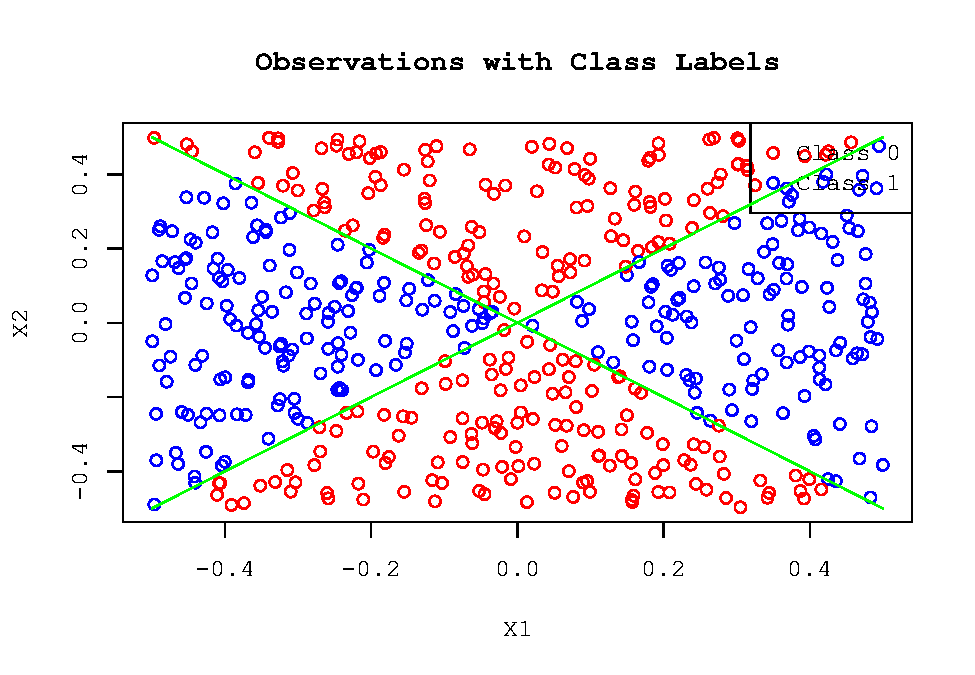
\includegraphics{ISLR4.7.10_files/figure-latex/unnamed-chunk-18-1.pdf}

\begin{enumerate}
\def\labelenumi{(\alph{enumi})}
\setcounter{enumi}{2}
\tightlist
\item
  Fit a logistic regression model to the data, using X1 and X2 as
  predictors.
\end{enumerate}

\begin{Shaded}
\begin{Highlighting}[]
\NormalTok{model }\OtherTok{=} \FunctionTok{glm}\NormalTok{(y }\SpecialCharTok{\textasciitilde{}}\NormalTok{ x1 }\SpecialCharTok{+}\NormalTok{ x2, }\AttributeTok{data =}\NormalTok{ data, }\AttributeTok{family =}\NormalTok{ binomial)}

\FunctionTok{summary}\NormalTok{(model)}
\end{Highlighting}
\end{Shaded}

\begin{verbatim}
## 
## Call:
## glm(formula = y ~ x1 + x2, family = binomial, data = data)
## 
## Coefficients:
##              Estimate Std. Error z value Pr(>|z|)
## (Intercept)  0.005622   0.089578   0.063    0.950
## x1          -0.316573   0.313418  -1.010    0.312
## x2           0.122073   0.315136   0.387    0.698
## 
## (Dispersion parameter for binomial family taken to be 1)
## 
##     Null deviance: 693.14  on 499  degrees of freedom
## Residual deviance: 691.98  on 497  degrees of freedom
## AIC: 697.98
## 
## Number of Fisher Scoring iterations: 3
\end{verbatim}

\begin{enumerate}
\def\labelenumi{(\alph{enumi})}
\setcounter{enumi}{3}
\tightlist
\item
  Apply this model to the training data in order to obtain a predicted
  class label for each training observation. Plot the observations,
  colored according to the predicted class labels. The decision boundary
  should be linear.
\end{enumerate}

\begin{Shaded}
\begin{Highlighting}[]
\NormalTok{data}\SpecialCharTok{$}\NormalTok{predicted\_class }\OtherTok{=} \FunctionTok{predict}\NormalTok{(model, }\AttributeTok{newdata =}\NormalTok{ data, }\AttributeTok{type =} \StringTok{"response"}\NormalTok{) }\SpecialCharTok{\textgreater{}=} \FloatTok{0.5}

\NormalTok{x1\_seq }\OtherTok{=} \FunctionTok{seq}\NormalTok{(}\SpecialCharTok{{-}}\FloatTok{0.5}\NormalTok{, }\FloatTok{0.5}\NormalTok{, }\AttributeTok{length.out =} \DecValTok{100}\NormalTok{)}
\NormalTok{x2\_seq }\OtherTok{=} \FunctionTok{seq}\NormalTok{(}\SpecialCharTok{{-}}\FloatTok{0.5}\NormalTok{, }\FloatTok{0.5}\NormalTok{, }\AttributeTok{length.out =} \DecValTok{100}\NormalTok{)}
\NormalTok{boundary }\OtherTok{=} \FunctionTok{matrix}\NormalTok{(}\DecValTok{0}\NormalTok{, }\AttributeTok{nrow =} \DecValTok{100}\NormalTok{, }\AttributeTok{ncol =} \DecValTok{100}\NormalTok{)}
\ControlFlowTok{for}\NormalTok{ (i }\ControlFlowTok{in} \DecValTok{1}\SpecialCharTok{:}\DecValTok{100}\NormalTok{) \{}
  \ControlFlowTok{for}\NormalTok{ (j }\ControlFlowTok{in} \DecValTok{1}\SpecialCharTok{:}\DecValTok{100}\NormalTok{) \{}
\NormalTok{    boundary[i, j] }\OtherTok{\textless{}{-}} \FunctionTok{predict}\NormalTok{(model, }\AttributeTok{newdata =} \FunctionTok{data.frame}\NormalTok{(}\AttributeTok{x1 =}\NormalTok{ x1\_seq[i], }\AttributeTok{x2 =}\NormalTok{ x2\_seq[j], }\AttributeTok{type =} \StringTok{"response"}\NormalTok{))}
\NormalTok{  \}}
\NormalTok{\}}
\FunctionTok{par}\NormalTok{(}\AttributeTok{oma =} \FunctionTok{c}\NormalTok{(}\DecValTok{0}\NormalTok{, }\DecValTok{0}\NormalTok{, }\DecValTok{0}\NormalTok{, }\DecValTok{8}\NormalTok{)) }
\FunctionTok{par}\NormalTok{(}\AttributeTok{family =} \StringTok{"mono"}\NormalTok{)}
\FunctionTok{plot}\NormalTok{(}\DecValTok{0}\NormalTok{, }\AttributeTok{type =} \StringTok{"n"}\NormalTok{, }\AttributeTok{xlim =} \FunctionTok{range}\NormalTok{(x1\_seq), }\AttributeTok{ylim =} \FunctionTok{range}\NormalTok{(x2\_seq), }\AttributeTok{xlab =} \StringTok{"X1"}\NormalTok{, }\AttributeTok{ylab =} \StringTok{"X2"}\NormalTok{, }\AttributeTok{main =} \StringTok{"Logistic Regression Model Predicted Result"}\NormalTok{)}

\NormalTok{custom\_palette }\OtherTok{=} \FunctionTok{colorRampPalette}\NormalTok{(}\FunctionTok{c}\NormalTok{(}\StringTok{"\#EEAAAA"}\NormalTok{, }\StringTok{"\#AAAAEE"}\NormalTok{))}
\FunctionTok{image}\NormalTok{(x1\_seq, x2\_seq, boundary, }\AttributeTok{col =} \FunctionTok{custom\_palette}\NormalTok{(}\DecValTok{50}\NormalTok{), }\AttributeTok{add =} \ConstantTok{TRUE}\NormalTok{)}

\FunctionTok{points}\NormalTok{(data}\SpecialCharTok{$}\NormalTok{x1, data}\SpecialCharTok{$}\NormalTok{x2, }\AttributeTok{col =} \FunctionTok{ifelse}\NormalTok{(data}\SpecialCharTok{$}\NormalTok{predicted\_class }\SpecialCharTok{==} \DecValTok{1}\NormalTok{, }\StringTok{"blue"}\NormalTok{, }\StringTok{"red"}\NormalTok{), }
       \AttributeTok{pch =}\NormalTok{ y }\SpecialCharTok{*} \DecValTok{4} \SpecialCharTok{+} \DecValTok{2}\NormalTok{, }\AttributeTok{cex =} \FloatTok{0.7}\NormalTok{)}
\FunctionTok{abline}\NormalTok{(}\FunctionTok{coef}\NormalTok{(model)[}\DecValTok{1}\NormalTok{] }\SpecialCharTok{/} \SpecialCharTok{{-}}\FunctionTok{coef}\NormalTok{(model)[}\DecValTok{3}\NormalTok{], }\FunctionTok{coef}\NormalTok{(model)[}\DecValTok{2}\NormalTok{] }\SpecialCharTok{/} \SpecialCharTok{{-}}\FunctionTok{coef}\NormalTok{(model)[}\DecValTok{3}\NormalTok{], }\AttributeTok{col =} \StringTok{"gold"}\NormalTok{, }\AttributeTok{lwd =} \DecValTok{2}\NormalTok{)}
\FunctionTok{curve}\NormalTok{(}\DecValTok{1}\SpecialCharTok{*}\NormalTok{x, }\AttributeTok{from =} \SpecialCharTok{{-}}\FloatTok{0.5}\NormalTok{, }\AttributeTok{to =} \FloatTok{0.5}\NormalTok{, }\AttributeTok{add =} \ConstantTok{TRUE}\NormalTok{, }\AttributeTok{col =} \StringTok{"green"}\NormalTok{,}\AttributeTok{lty =} \DecValTok{2}\NormalTok{, }\AttributeTok{lwd =} \DecValTok{2}\NormalTok{)}
\FunctionTok{curve}\NormalTok{(}\SpecialCharTok{{-}}\DecValTok{1}\SpecialCharTok{*}\NormalTok{x, }\AttributeTok{from =} \SpecialCharTok{{-}}\FloatTok{0.5}\NormalTok{, }\AttributeTok{to =} \FloatTok{0.5}\NormalTok{, }\AttributeTok{add =} \ConstantTok{TRUE}\NormalTok{, }\AttributeTok{col =} \StringTok{"green"}\NormalTok{, }\AttributeTok{lty =} \DecValTok{2}\NormalTok{, }\AttributeTok{lwd =} \DecValTok{2}\NormalTok{)}
\FunctionTok{par}\NormalTok{(}\AttributeTok{xpd =} \ConstantTok{NA}\NormalTok{)}

\FunctionTok{legend}\NormalTok{(}\AttributeTok{x =} \FloatTok{0.55}\NormalTok{, }\AttributeTok{y =} \FloatTok{0.5}\NormalTok{, }
       \AttributeTok{legend =} \FunctionTok{c}\NormalTok{(}\StringTok{"Predicted Class 0"}\NormalTok{, }\StringTok{"Predicted Class 1"}\NormalTok{, }
                  \StringTok{"Actual Class 0"}\NormalTok{, }\StringTok{"Actual Class 1"}\NormalTok{, }\StringTok{"Predicted Boundary"}\NormalTok{, }\StringTok{"Actual Boundary"}\NormalTok{), }
       \AttributeTok{col =} \FunctionTok{c}\NormalTok{(}\StringTok{"red"}\NormalTok{, }\StringTok{"blue"}\NormalTok{, }\StringTok{"black"}\NormalTok{, }\StringTok{"black"}\NormalTok{, }\StringTok{"gold"}\NormalTok{, }\StringTok{"green"}\NormalTok{), }
       \AttributeTok{pch =} \FunctionTok{c}\NormalTok{(}\DecValTok{4}\NormalTok{, }\DecValTok{4}\NormalTok{, }\DecValTok{2}\NormalTok{, }\DecValTok{6}\NormalTok{, }\ConstantTok{NA}\NormalTok{, }\ConstantTok{NA}\NormalTok{),}
       \AttributeTok{lwd =} \FunctionTok{c}\NormalTok{(}\ConstantTok{NA}\NormalTok{, }\ConstantTok{NA}\NormalTok{, }\ConstantTok{NA}\NormalTok{, }\ConstantTok{NA}\NormalTok{, }\DecValTok{1}\NormalTok{, }\DecValTok{1}\NormalTok{),}
       \AttributeTok{lty =} \FunctionTok{c}\NormalTok{(}\DecValTok{1}\NormalTok{, }\DecValTok{1}\NormalTok{, }\DecValTok{1}\NormalTok{, }\DecValTok{1}\NormalTok{, }\DecValTok{1}\NormalTok{, }\DecValTok{2}\NormalTok{),}
       \AttributeTok{cex =} \FloatTok{0.8}
\NormalTok{       )}
\end{Highlighting}
\end{Shaded}

\includegraphics{ISLR4.7.10_files/figure-latex/unnamed-chunk-20-1.pdf}

\begin{enumerate}
\def\labelenumi{(\alph{enumi})}
\setcounter{enumi}{4}
\tightlist
\item
  Now fit a logistic regression model to the data using non-linear
  functions of X1 and X2 as predictors (e.g.~X\_1\^{}2 , X1×X2, log(X2),
  and so forth).
\end{enumerate}

\begin{Shaded}
\begin{Highlighting}[]
\NormalTok{data}\SpecialCharTok{$}\NormalTok{X1\_squared }\OtherTok{\textless{}{-}}\NormalTok{ data}\SpecialCharTok{$}\NormalTok{x1}\SpecialCharTok{\^{}}\DecValTok{2}
\NormalTok{data}\SpecialCharTok{$}\NormalTok{X1\_times\_X2 }\OtherTok{\textless{}{-}}\NormalTok{ data}\SpecialCharTok{$}\NormalTok{x1 }\SpecialCharTok{*}\NormalTok{ data}\SpecialCharTok{$}\NormalTok{x2}
\NormalTok{data}\SpecialCharTok{$}\NormalTok{log\_X2\_squared }\OtherTok{\textless{}{-}} \FunctionTok{log}\NormalTok{(data}\SpecialCharTok{$}\NormalTok{x2}\SpecialCharTok{\^{}}\DecValTok{2}\NormalTok{)}

\NormalTok{model\_nonlinear }\OtherTok{\textless{}{-}} \FunctionTok{glm}\NormalTok{(y }\SpecialCharTok{\textasciitilde{}}\NormalTok{ X1\_squared }\SpecialCharTok{+}\NormalTok{ X1\_times\_X2 }\SpecialCharTok{+}\NormalTok{ log\_X2\_squared, }\AttributeTok{data =}\NormalTok{ data, }\AttributeTok{family =}\NormalTok{ binomial)}

\NormalTok{data}\SpecialCharTok{$}\NormalTok{predicted\_class }\OtherTok{=} \FunctionTok{predict}\NormalTok{(model\_nonlinear, }\AttributeTok{newdata =}\NormalTok{ data, }\AttributeTok{type =} \StringTok{"response"}\NormalTok{) }\SpecialCharTok{\textgreater{}=} \FloatTok{0.5}

\FunctionTok{summary}\NormalTok{(model\_nonlinear)}
\end{Highlighting}
\end{Shaded}

\begin{verbatim}
## 
## Call:
## glm(formula = y ~ X1_squared + X1_times_X2 + log_X2_squared, 
##     family = binomial, data = data)
## 
## Coefficients:
##                Estimate Std. Error z value Pr(>|z|)    
## (Intercept)    -11.2188     1.1471  -9.780   <2e-16 ***
## X1_squared      47.7221     4.9685   9.605   <2e-16 ***
## X1_times_X2      0.9873     1.8845   0.524      0.6    
## log_X2_squared  -2.3545     0.2555  -9.214   <2e-16 ***
## ---
## Signif. codes:  0 '***' 0.001 '**' 0.01 '*' 0.05 '.' 0.1 ' ' 1
## 
## (Dispersion parameter for binomial family taken to be 1)
## 
##     Null deviance: 693.14  on 499  degrees of freedom
## Residual deviance: 208.35  on 496  degrees of freedom
## AIC: 216.35
## 
## Number of Fisher Scoring iterations: 7
\end{verbatim}

\begin{enumerate}
\def\labelenumi{(\alph{enumi})}
\setcounter{enumi}{5}
\tightlist
\item
  Apply this model to the training data in order to obtain a predicted
  class label for each training observation. Plot the observations,
  colored according to the predicted class labels. The decision boundary
  should be obviously non-linear. If it is not, then repeat (a)-(e)
  until you come up with an example in which the predicted class labels
  are obviously non-linear.
\end{enumerate}

\begin{Shaded}
\begin{Highlighting}[]
\NormalTok{x1\_seq }\OtherTok{=} \FunctionTok{seq}\NormalTok{(}\SpecialCharTok{{-}}\FloatTok{0.5}\NormalTok{, }\FloatTok{0.5}\NormalTok{, }\AttributeTok{length.out =} \DecValTok{100}\NormalTok{)}
\NormalTok{x2\_seq }\OtherTok{=} \FunctionTok{seq}\NormalTok{(}\SpecialCharTok{{-}}\FloatTok{0.5}\NormalTok{, }\FloatTok{0.5}\NormalTok{, }\AttributeTok{length.out =} \DecValTok{100}\NormalTok{)}
\NormalTok{boundary }\OtherTok{=} \FunctionTok{matrix}\NormalTok{(}\DecValTok{0}\NormalTok{, }\AttributeTok{nrow =} \DecValTok{100}\NormalTok{, }\AttributeTok{ncol =} \DecValTok{100}\NormalTok{)}
\ControlFlowTok{for}\NormalTok{ (i }\ControlFlowTok{in} \DecValTok{1}\SpecialCharTok{:}\DecValTok{100}\NormalTok{) \{}
  \ControlFlowTok{for}\NormalTok{ (j }\ControlFlowTok{in} \DecValTok{1}\SpecialCharTok{:}\DecValTok{100}\NormalTok{) \{}
\NormalTok{    boundary[i, j] }\OtherTok{\textless{}{-}} \FunctionTok{predict}\NormalTok{(model\_nonlinear, }\AttributeTok{newdata =} \FunctionTok{data.frame}\NormalTok{(}\AttributeTok{X1\_squared =}\NormalTok{ x1\_seq[i]}\SpecialCharTok{\^{}}\DecValTok{2}\NormalTok{, }\AttributeTok{X1\_times\_X2 =}\NormalTok{ x1\_seq[i] }\SpecialCharTok{*}\NormalTok{ x2\_seq[j], }\AttributeTok{log\_X2\_squared =} \FunctionTok{log}\NormalTok{(x2\_seq[j]}\SpecialCharTok{\^{}}\DecValTok{2}\NormalTok{)), }\AttributeTok{type =} \StringTok{"response"}\NormalTok{)}
\NormalTok{  \}}
\NormalTok{\}}
\FunctionTok{par}\NormalTok{(}\AttributeTok{oma =} \FunctionTok{c}\NormalTok{(}\DecValTok{0}\NormalTok{, }\DecValTok{0}\NormalTok{, }\DecValTok{0}\NormalTok{, }\DecValTok{8}\NormalTok{)) }
\FunctionTok{par}\NormalTok{(}\AttributeTok{family =} \StringTok{"mono"}\NormalTok{)}
\FunctionTok{plot}\NormalTok{(}\DecValTok{0}\NormalTok{, }\AttributeTok{type =} \StringTok{"n"}\NormalTok{, }\AttributeTok{xlim =} \FunctionTok{range}\NormalTok{(x1\_seq), }\AttributeTok{ylim =} \FunctionTok{range}\NormalTok{(x2\_seq), }\AttributeTok{xlab =} \StringTok{"X1"}\NormalTok{, }\AttributeTok{ylab =} \StringTok{"X2"}\NormalTok{, }\AttributeTok{main =} \StringTok{"Non{-}linear Logistic Regression Model Predicted Result"}\NormalTok{)}

\NormalTok{custom\_palette }\OtherTok{=} \FunctionTok{colorRampPalette}\NormalTok{(}\FunctionTok{c}\NormalTok{(}\StringTok{"\#EEAAAA"}\NormalTok{, }\StringTok{"\#AAAAEE"}\NormalTok{))}
\FunctionTok{image}\NormalTok{(x1\_seq, x2\_seq, boundary, }\AttributeTok{col =} \FunctionTok{custom\_palette}\NormalTok{(}\DecValTok{50}\NormalTok{), }\AttributeTok{add =} \ConstantTok{TRUE}\NormalTok{)}

\FunctionTok{points}\NormalTok{(data}\SpecialCharTok{$}\NormalTok{x1, data}\SpecialCharTok{$}\NormalTok{x2, }\AttributeTok{col =} \FunctionTok{ifelse}\NormalTok{(data}\SpecialCharTok{$}\NormalTok{predicted\_class }\SpecialCharTok{==} \DecValTok{1}\NormalTok{, }\StringTok{"blue"}\NormalTok{, }\StringTok{"red"}\NormalTok{), }
       \AttributeTok{pch =}\NormalTok{ y }\SpecialCharTok{*} \DecValTok{4} \SpecialCharTok{+} \DecValTok{2}\NormalTok{, }\AttributeTok{cex =} \FloatTok{0.7}\NormalTok{)}

\FunctionTok{curve}\NormalTok{(}\DecValTok{1}\SpecialCharTok{*}\NormalTok{x, }\AttributeTok{from =} \SpecialCharTok{{-}}\FloatTok{0.5}\NormalTok{, }\AttributeTok{to =} \FloatTok{0.5}\NormalTok{, }\AttributeTok{add =} \ConstantTok{TRUE}\NormalTok{, }\AttributeTok{col =} \StringTok{"green"}\NormalTok{,}\AttributeTok{lty =} \DecValTok{2}\NormalTok{, }\AttributeTok{lwd =} \DecValTok{2}\NormalTok{)}
\FunctionTok{curve}\NormalTok{(}\SpecialCharTok{{-}}\DecValTok{1}\SpecialCharTok{*}\NormalTok{x, }\AttributeTok{from =} \SpecialCharTok{{-}}\FloatTok{0.5}\NormalTok{, }\AttributeTok{to =} \FloatTok{0.5}\NormalTok{, }\AttributeTok{add =} \ConstantTok{TRUE}\NormalTok{, }\AttributeTok{col =} \StringTok{"green"}\NormalTok{, }\AttributeTok{lty =} \DecValTok{2}\NormalTok{, }\AttributeTok{lwd =} \DecValTok{2}\NormalTok{)}
\FunctionTok{contour}\NormalTok{(x1\_seq, x2\_seq, boundary, }\AttributeTok{levels =} \FloatTok{0.5}\NormalTok{, }\AttributeTok{drawlabels =} \ConstantTok{FALSE}\NormalTok{, }\AttributeTok{col =} \StringTok{"cyan"}\NormalTok{, }\AttributeTok{add =} \ConstantTok{TRUE}\NormalTok{)}
\FunctionTok{par}\NormalTok{(}\AttributeTok{xpd =} \ConstantTok{NA}\NormalTok{)}

\FunctionTok{legend}\NormalTok{(}\AttributeTok{x =} \FloatTok{0.55}\NormalTok{, }\AttributeTok{y =} \FloatTok{0.5}\NormalTok{, }
       \AttributeTok{legend =} \FunctionTok{c}\NormalTok{(}\StringTok{"Predicted Class 0"}\NormalTok{, }\StringTok{"Predicted Class 1"}\NormalTok{, }
                  \StringTok{"Actual Class 0"}\NormalTok{, }\StringTok{"Actual Class 1"}\NormalTok{, }\StringTok{"Predicted Boundary"}\NormalTok{, }\StringTok{"Actual Boundary"}\NormalTok{), }
       \AttributeTok{col =} \FunctionTok{c}\NormalTok{(}\StringTok{"red"}\NormalTok{, }\StringTok{"blue"}\NormalTok{, }\StringTok{"black"}\NormalTok{, }\StringTok{"black"}\NormalTok{, }\StringTok{"cyan"}\NormalTok{, }\StringTok{"green"}\NormalTok{), }
       \AttributeTok{pch =} \FunctionTok{c}\NormalTok{(}\DecValTok{4}\NormalTok{, }\DecValTok{4}\NormalTok{, }\DecValTok{2}\NormalTok{, }\DecValTok{6}\NormalTok{, }\ConstantTok{NA}\NormalTok{, }\ConstantTok{NA}\NormalTok{),}
       \AttributeTok{lwd =} \FunctionTok{c}\NormalTok{(}\ConstantTok{NA}\NormalTok{, }\ConstantTok{NA}\NormalTok{, }\ConstantTok{NA}\NormalTok{, }\ConstantTok{NA}\NormalTok{, }\DecValTok{1}\NormalTok{, }\DecValTok{1}\NormalTok{),}
       \AttributeTok{lty =} \FunctionTok{c}\NormalTok{(}\DecValTok{1}\NormalTok{, }\DecValTok{1}\NormalTok{, }\DecValTok{1}\NormalTok{, }\DecValTok{1}\NormalTok{, }\DecValTok{1}\NormalTok{, }\DecValTok{2}\NormalTok{),}
       \AttributeTok{cex =} \FloatTok{0.8}
\NormalTok{       )}
\end{Highlighting}
\end{Shaded}

\includegraphics{ISLR4.7.10_files/figure-latex/unnamed-chunk-22-1.pdf}

\begin{enumerate}
\def\labelenumi{(\alph{enumi})}
\setcounter{enumi}{6}
\tightlist
\item
  Fit a support vector classifier to the data with X1 and X2 as
  predictors. Obtain a class prediction for each training observation.
  Plot the observations, colored according to the predicted class
  labels.
\end{enumerate}

\begin{Shaded}
\begin{Highlighting}[]
\NormalTok{svm\_model }\OtherTok{\textless{}{-}} \FunctionTok{svm}\NormalTok{(y }\SpecialCharTok{\textasciitilde{}}\NormalTok{ ., }\AttributeTok{data =} \FunctionTok{data.frame}\NormalTok{(data[, }\FunctionTok{c}\NormalTok{(}\StringTok{"x1"}\NormalTok{, }\StringTok{"x2"}\NormalTok{)]), }\AttributeTok{kernel =} \StringTok{"linear"}\NormalTok{, }\AttributeTok{cost =} \DecValTok{5}\NormalTok{, }\AttributeTok{scale =} \ConstantTok{FALSE}\NormalTok{)}

\NormalTok{data}\SpecialCharTok{$}\NormalTok{predicted\_svm }\OtherTok{\textless{}{-}} \FunctionTok{predict}\NormalTok{(svm\_model, }\FunctionTok{data.frame}\NormalTok{(data[, }\FunctionTok{c}\NormalTok{(}\StringTok{"x1"}\NormalTok{, }\StringTok{"x2"}\NormalTok{)]), }\AttributeTok{type =} \StringTok{"response"}\NormalTok{) }\SpecialCharTok{\textgreater{}=} \FloatTok{0.5}

\NormalTok{x1\_seq }\OtherTok{=} \FunctionTok{seq}\NormalTok{(}\SpecialCharTok{{-}}\FloatTok{0.5}\NormalTok{, }\FloatTok{0.5}\NormalTok{, }\AttributeTok{length.out =} \DecValTok{100}\NormalTok{)}
\NormalTok{x2\_seq }\OtherTok{=} \FunctionTok{seq}\NormalTok{(}\SpecialCharTok{{-}}\FloatTok{0.5}\NormalTok{, }\FloatTok{0.5}\NormalTok{, }\AttributeTok{length.out =} \DecValTok{100}\NormalTok{)}
\NormalTok{boundary }\OtherTok{=} \FunctionTok{matrix}\NormalTok{(}\DecValTok{0}\NormalTok{, }\AttributeTok{nrow =} \DecValTok{100}\NormalTok{, }\AttributeTok{ncol =} \DecValTok{100}\NormalTok{)}
\ControlFlowTok{for}\NormalTok{ (i }\ControlFlowTok{in} \DecValTok{1}\SpecialCharTok{:}\DecValTok{100}\NormalTok{) \{}
  \ControlFlowTok{for}\NormalTok{ (j }\ControlFlowTok{in} \DecValTok{1}\SpecialCharTok{:}\DecValTok{100}\NormalTok{) \{}
\NormalTok{    boundary[i, j] }\OtherTok{\textless{}{-}} \FunctionTok{predict}\NormalTok{(svm\_model, }\AttributeTok{newdata =} \FunctionTok{data.frame}\NormalTok{(}\AttributeTok{x1 =}\NormalTok{ x1\_seq[i], }\AttributeTok{x2 =}\NormalTok{ x2\_seq[j]), }\AttributeTok{type =} \StringTok{"response"}\NormalTok{)}
\NormalTok{  \}}
\NormalTok{\}}
\FunctionTok{par}\NormalTok{(}\AttributeTok{oma =} \FunctionTok{c}\NormalTok{(}\DecValTok{0}\NormalTok{, }\DecValTok{0}\NormalTok{, }\DecValTok{0}\NormalTok{, }\DecValTok{8}\NormalTok{)) }
\FunctionTok{par}\NormalTok{(}\AttributeTok{family =} \StringTok{"mono"}\NormalTok{)}
\FunctionTok{plot}\NormalTok{(}\DecValTok{0}\NormalTok{, }\AttributeTok{type =} \StringTok{"n"}\NormalTok{, }\AttributeTok{xlim =} \FunctionTok{range}\NormalTok{(x1\_seq), }\AttributeTok{ylim =} \FunctionTok{range}\NormalTok{(x2\_seq), }\AttributeTok{xlab =} \StringTok{"X1"}\NormalTok{, }\AttributeTok{ylab =} \StringTok{"X2"}\NormalTok{, }\AttributeTok{main =} \StringTok{"SVC Predicted Results"}\NormalTok{)}

\NormalTok{custom\_palette }\OtherTok{=} \FunctionTok{colorRampPalette}\NormalTok{(}\FunctionTok{c}\NormalTok{(}\StringTok{"\#EEAAAA"}\NormalTok{, }\StringTok{"\#AAAAEE"}\NormalTok{))}
\FunctionTok{image}\NormalTok{(x1\_seq, x2\_seq, boundary, }\AttributeTok{col =} \FunctionTok{custom\_palette}\NormalTok{(}\DecValTok{50}\NormalTok{), }\AttributeTok{add =} \ConstantTok{TRUE}\NormalTok{)}

\FunctionTok{points}\NormalTok{(data}\SpecialCharTok{$}\NormalTok{x1, data}\SpecialCharTok{$}\NormalTok{x2, }\AttributeTok{col =} \FunctionTok{ifelse}\NormalTok{(data}\SpecialCharTok{$}\NormalTok{predicted\_svm }\SpecialCharTok{==} \DecValTok{1}\NormalTok{, }\StringTok{"blue"}\NormalTok{, }\StringTok{"red"}\NormalTok{), }
       \AttributeTok{pch =}\NormalTok{ y }\SpecialCharTok{*} \DecValTok{4} \SpecialCharTok{+} \DecValTok{2}\NormalTok{, }\AttributeTok{cex =} \FloatTok{0.7}\NormalTok{)}

\FunctionTok{curve}\NormalTok{(}\DecValTok{1}\SpecialCharTok{*}\NormalTok{x, }\AttributeTok{from =} \SpecialCharTok{{-}}\FloatTok{0.5}\NormalTok{, }\AttributeTok{to =} \FloatTok{0.5}\NormalTok{, }\AttributeTok{add =} \ConstantTok{TRUE}\NormalTok{, }\AttributeTok{col =} \StringTok{"green"}\NormalTok{,}\AttributeTok{lty =} \DecValTok{2}\NormalTok{, }\AttributeTok{lwd =} \DecValTok{2}\NormalTok{)}
\FunctionTok{curve}\NormalTok{(}\SpecialCharTok{{-}}\DecValTok{1}\SpecialCharTok{*}\NormalTok{x, }\AttributeTok{from =} \SpecialCharTok{{-}}\FloatTok{0.5}\NormalTok{, }\AttributeTok{to =} \FloatTok{0.5}\NormalTok{, }\AttributeTok{add =} \ConstantTok{TRUE}\NormalTok{, }\AttributeTok{col =} \StringTok{"green"}\NormalTok{, }\AttributeTok{lty =} \DecValTok{2}\NormalTok{, }\AttributeTok{lwd =} \DecValTok{2}\NormalTok{)}
\FunctionTok{contour}\NormalTok{(x1\_seq, x2\_seq, boundary, }\AttributeTok{levels =} \FloatTok{0.5}\NormalTok{, }\AttributeTok{drawlabels =} \ConstantTok{FALSE}\NormalTok{, }\AttributeTok{col =} \StringTok{"cyan"}\NormalTok{, }\AttributeTok{add =} \ConstantTok{TRUE}\NormalTok{)}
\FunctionTok{par}\NormalTok{(}\AttributeTok{xpd =} \ConstantTok{NA}\NormalTok{)}

\FunctionTok{legend}\NormalTok{(}\AttributeTok{x =} \FloatTok{0.55}\NormalTok{, }\AttributeTok{y =} \FloatTok{0.5}\NormalTok{, }
       \AttributeTok{legend =} \FunctionTok{c}\NormalTok{(}\StringTok{"Predicted Class 0"}\NormalTok{, }\StringTok{"Predicted Class 1"}\NormalTok{, }
                  \StringTok{"Actual Class 0"}\NormalTok{, }\StringTok{"Actual Class 1"}\NormalTok{, }\StringTok{"Predicted Boundary"}\NormalTok{, }\StringTok{"Actual Boundary"}\NormalTok{), }
       \AttributeTok{col =} \FunctionTok{c}\NormalTok{(}\StringTok{"red"}\NormalTok{, }\StringTok{"blue"}\NormalTok{, }\StringTok{"black"}\NormalTok{, }\StringTok{"black"}\NormalTok{, }\StringTok{"cyan"}\NormalTok{, }\StringTok{"green"}\NormalTok{), }
       \AttributeTok{pch =} \FunctionTok{c}\NormalTok{(}\DecValTok{4}\NormalTok{, }\DecValTok{4}\NormalTok{, }\DecValTok{2}\NormalTok{, }\DecValTok{6}\NormalTok{, }\ConstantTok{NA}\NormalTok{, }\ConstantTok{NA}\NormalTok{),}
       \AttributeTok{lwd =} \FunctionTok{c}\NormalTok{(}\ConstantTok{NA}\NormalTok{, }\ConstantTok{NA}\NormalTok{, }\ConstantTok{NA}\NormalTok{, }\ConstantTok{NA}\NormalTok{, }\DecValTok{1}\NormalTok{, }\DecValTok{1}\NormalTok{),}
       \AttributeTok{lty =} \FunctionTok{c}\NormalTok{(}\DecValTok{1}\NormalTok{, }\DecValTok{1}\NormalTok{, }\DecValTok{1}\NormalTok{, }\DecValTok{1}\NormalTok{, }\DecValTok{1}\NormalTok{, }\DecValTok{2}\NormalTok{),}
       \AttributeTok{cex =} \FloatTok{0.8}
\NormalTok{       )}
\end{Highlighting}
\end{Shaded}

\includegraphics{ISLR4.7.10_files/figure-latex/unnamed-chunk-23-1.pdf}

\begin{enumerate}
\def\labelenumi{(\alph{enumi})}
\setcounter{enumi}{7}
\tightlist
\item
  Fit a SVM using a non-linear kernel to the data. Obtain a class
  prediction for each training observation. Plot the observations,
  colored according to the predicted class labels.
\end{enumerate}

\begin{Shaded}
\begin{Highlighting}[]
\NormalTok{X }\OtherTok{=}\NormalTok{ data[, }\FunctionTok{c}\NormalTok{(}\StringTok{"x1"}\NormalTok{, }\StringTok{"x2"}\NormalTok{)]}

\NormalTok{svm\_model }\OtherTok{=} \FunctionTok{svm}\NormalTok{(y }\SpecialCharTok{\textasciitilde{}}\NormalTok{ ., }\AttributeTok{data =} \FunctionTok{data.frame}\NormalTok{(X, y), }\AttributeTok{kernel =} \StringTok{"radial"}\NormalTok{)}

\NormalTok{predicted\_classes }\OtherTok{\textless{}{-}} \FunctionTok{predict}\NormalTok{(svm\_model, }\FunctionTok{data.frame}\NormalTok{(X)) }\SpecialCharTok{\textgreater{}=} \FloatTok{0.5}

\NormalTok{x1\_seq }\OtherTok{=} \FunctionTok{seq}\NormalTok{(}\SpecialCharTok{{-}}\FloatTok{0.5}\NormalTok{, }\FloatTok{0.5}\NormalTok{, }\AttributeTok{length.out =} \DecValTok{100}\NormalTok{)}
\NormalTok{x2\_seq }\OtherTok{=} \FunctionTok{seq}\NormalTok{(}\SpecialCharTok{{-}}\FloatTok{0.5}\NormalTok{, }\FloatTok{0.5}\NormalTok{, }\AttributeTok{length.out =} \DecValTok{100}\NormalTok{)}
\NormalTok{boundary }\OtherTok{=} \FunctionTok{matrix}\NormalTok{(}\DecValTok{0}\NormalTok{, }\AttributeTok{nrow =} \DecValTok{100}\NormalTok{, }\AttributeTok{ncol =} \DecValTok{100}\NormalTok{)}
\ControlFlowTok{for}\NormalTok{ (i }\ControlFlowTok{in} \DecValTok{1}\SpecialCharTok{:}\DecValTok{100}\NormalTok{) \{}
  \ControlFlowTok{for}\NormalTok{ (j }\ControlFlowTok{in} \DecValTok{1}\SpecialCharTok{:}\DecValTok{100}\NormalTok{) \{}
\NormalTok{    boundary[i, j] }\OtherTok{\textless{}{-}} \FunctionTok{predict}\NormalTok{(svm\_model, }\AttributeTok{newdata =} \FunctionTok{data.frame}\NormalTok{(}\AttributeTok{x1 =}\NormalTok{ x1\_seq[i], }\AttributeTok{x2 =}\NormalTok{ x2\_seq[j]), }\AttributeTok{type =} \StringTok{"response"}\NormalTok{)}
\NormalTok{  \}}
\NormalTok{\}}
\FunctionTok{par}\NormalTok{(}\AttributeTok{oma =} \FunctionTok{c}\NormalTok{(}\DecValTok{0}\NormalTok{, }\DecValTok{0}\NormalTok{, }\DecValTok{0}\NormalTok{, }\DecValTok{8}\NormalTok{)) }
\FunctionTok{par}\NormalTok{(}\AttributeTok{family =} \StringTok{"mono"}\NormalTok{)}
\FunctionTok{plot}\NormalTok{(}\DecValTok{0}\NormalTok{, }\AttributeTok{type =} \StringTok{"n"}\NormalTok{, }\AttributeTok{xlim =} \FunctionTok{range}\NormalTok{(x1\_seq), }\AttributeTok{ylim =} \FunctionTok{range}\NormalTok{(x2\_seq), }\AttributeTok{xlab =} \StringTok{"X1"}\NormalTok{, }\AttributeTok{ylab =} \StringTok{"X2"}\NormalTok{, }\AttributeTok{main =} \StringTok{"SVM with Non{-}linear Kernel Predicted Results"}\NormalTok{)}

\NormalTok{custom\_palette }\OtherTok{=} \FunctionTok{colorRampPalette}\NormalTok{(}\FunctionTok{c}\NormalTok{(}\StringTok{"\#EEAAAA"}\NormalTok{, }\StringTok{"\#AAAAEE"}\NormalTok{))}
\FunctionTok{image}\NormalTok{(x1\_seq, x2\_seq, boundary, }\AttributeTok{col =} \FunctionTok{custom\_palette}\NormalTok{(}\DecValTok{50}\NormalTok{), }\AttributeTok{add =} \ConstantTok{TRUE}\NormalTok{)}

\FunctionTok{points}\NormalTok{(data}\SpecialCharTok{$}\NormalTok{x1, data}\SpecialCharTok{$}\NormalTok{x2, }\AttributeTok{col =} \FunctionTok{ifelse}\NormalTok{(predicted\_classes }\SpecialCharTok{==} \DecValTok{1}\NormalTok{, }\StringTok{"blue"}\NormalTok{, }\StringTok{"red"}\NormalTok{), }
       \AttributeTok{pch =}\NormalTok{ y }\SpecialCharTok{*} \DecValTok{4} \SpecialCharTok{+} \DecValTok{2}\NormalTok{, }\AttributeTok{cex =} \FloatTok{0.7}\NormalTok{)}

\FunctionTok{curve}\NormalTok{(}\DecValTok{1}\SpecialCharTok{*}\NormalTok{x, }\AttributeTok{from =} \SpecialCharTok{{-}}\FloatTok{0.5}\NormalTok{, }\AttributeTok{to =} \FloatTok{0.5}\NormalTok{, }\AttributeTok{add =} \ConstantTok{TRUE}\NormalTok{, }\AttributeTok{col =} \StringTok{"green"}\NormalTok{,}\AttributeTok{lty =} \DecValTok{2}\NormalTok{, }\AttributeTok{lwd =} \DecValTok{2}\NormalTok{)}
\FunctionTok{curve}\NormalTok{(}\SpecialCharTok{{-}}\DecValTok{1}\SpecialCharTok{*}\NormalTok{x, }\AttributeTok{from =} \SpecialCharTok{{-}}\FloatTok{0.5}\NormalTok{, }\AttributeTok{to =} \FloatTok{0.5}\NormalTok{, }\AttributeTok{add =} \ConstantTok{TRUE}\NormalTok{, }\AttributeTok{col =} \StringTok{"green"}\NormalTok{, }\AttributeTok{lty =} \DecValTok{2}\NormalTok{, }\AttributeTok{lwd =} \DecValTok{2}\NormalTok{)}
\FunctionTok{contour}\NormalTok{(x1\_seq, x2\_seq, boundary, }\AttributeTok{levels =} \FloatTok{0.5}\NormalTok{, }\AttributeTok{drawlabels =} \ConstantTok{FALSE}\NormalTok{, }\AttributeTok{col =} \StringTok{"cyan"}\NormalTok{, }\AttributeTok{add =} \ConstantTok{TRUE}\NormalTok{)}
\FunctionTok{par}\NormalTok{(}\AttributeTok{xpd =} \ConstantTok{NA}\NormalTok{)}

\FunctionTok{legend}\NormalTok{(}\AttributeTok{x =} \FloatTok{0.55}\NormalTok{, }\AttributeTok{y =} \FloatTok{0.5}\NormalTok{, }
       \AttributeTok{legend =} \FunctionTok{c}\NormalTok{(}\StringTok{"Predicted Class 0"}\NormalTok{, }\StringTok{"Predicted Class 1"}\NormalTok{, }
                  \StringTok{"Actual Class 0"}\NormalTok{, }\StringTok{"Actual Class 1"}\NormalTok{, }\StringTok{"Predicted Boundary"}\NormalTok{, }\StringTok{"Actual Boundary"}\NormalTok{), }
       \AttributeTok{col =} \FunctionTok{c}\NormalTok{(}\StringTok{"red"}\NormalTok{, }\StringTok{"blue"}\NormalTok{, }\StringTok{"black"}\NormalTok{, }\StringTok{"black"}\NormalTok{, }\StringTok{"cyan"}\NormalTok{, }\StringTok{"green"}\NormalTok{), }
       \AttributeTok{pch =} \FunctionTok{c}\NormalTok{(}\DecValTok{4}\NormalTok{, }\DecValTok{4}\NormalTok{, }\DecValTok{2}\NormalTok{, }\DecValTok{6}\NormalTok{, }\ConstantTok{NA}\NormalTok{, }\ConstantTok{NA}\NormalTok{),}
       \AttributeTok{lwd =} \FunctionTok{c}\NormalTok{(}\ConstantTok{NA}\NormalTok{, }\ConstantTok{NA}\NormalTok{, }\ConstantTok{NA}\NormalTok{, }\ConstantTok{NA}\NormalTok{, }\DecValTok{1}\NormalTok{, }\DecValTok{1}\NormalTok{),}
       \AttributeTok{lty =} \FunctionTok{c}\NormalTok{(}\DecValTok{1}\NormalTok{, }\DecValTok{1}\NormalTok{, }\DecValTok{1}\NormalTok{, }\DecValTok{1}\NormalTok{, }\DecValTok{1}\NormalTok{, }\DecValTok{2}\NormalTok{),}
       \AttributeTok{cex =} \FloatTok{0.8}
\NormalTok{       )}
\end{Highlighting}
\end{Shaded}

\includegraphics{ISLR4.7.10_files/figure-latex/unnamed-chunk-24-1.pdf}

\begin{enumerate}
\def\labelenumi{(\roman{enumi})}
\tightlist
\item
  Comment on your results.
\end{enumerate}

All non-linear models applied in this experiment work well, while linear
models cannot fit the quadratic boundary well. Modifications of import
non-linear kernel is significant to the quadratic boundary fitting.

\textbf{ISLR Section 9.3.3 Reproduced}

\begin{Shaded}
\begin{Highlighting}[]
\NormalTok{heart\_data }\OtherTok{=} \FunctionTok{read.csv}\NormalTok{(}\StringTok{"Heart.csv"}\NormalTok{)}

\NormalTok{heart\_data }\OtherTok{=} \FunctionTok{na.omit}\NormalTok{(heart\_data)}

\NormalTok{heart\_data}\SpecialCharTok{$}\NormalTok{AHD[heart\_data}\SpecialCharTok{$}\NormalTok{AHD }\SpecialCharTok{==} \StringTok{"Yes"}\NormalTok{] }\OtherTok{=} \DecValTok{1}
\NormalTok{heart\_data}\SpecialCharTok{$}\NormalTok{AHD[heart\_data}\SpecialCharTok{$}\NormalTok{AHD }\SpecialCharTok{==} \StringTok{"No"}\NormalTok{] }\OtherTok{=} \DecValTok{0}
\NormalTok{heart\_data}\SpecialCharTok{$}\NormalTok{AHD }\OtherTok{=} \FunctionTok{as.numeric}\NormalTok{(heart\_data}\SpecialCharTok{$}\NormalTok{AHD)}


\FunctionTok{set.seed}\NormalTok{(}\DecValTok{114514}\NormalTok{)}

\NormalTok{train\_indices }\OtherTok{=} \FunctionTok{sample}\NormalTok{(}\DecValTok{1} \SpecialCharTok{:} \FunctionTok{nrow}\NormalTok{(heart\_data), }\DecValTok{207}\NormalTok{)}
\NormalTok{train\_data }\OtherTok{=}\NormalTok{ heart\_data[train\_indices, ]}
\NormalTok{test\_data }\OtherTok{=}\NormalTok{ heart\_data[}\SpecialCharTok{{-}}\NormalTok{train\_indices, ]}

\NormalTok{lda\_model }\OtherTok{=} \FunctionTok{lda}\NormalTok{(AHD }\SpecialCharTok{\textasciitilde{}}\NormalTok{ .}\SpecialCharTok{{-}}\NormalTok{X, }\AttributeTok{data =}\NormalTok{ train\_data)}

\NormalTok{svm\_linear\_model }\OtherTok{=} \FunctionTok{svm}\NormalTok{(AHD}\SpecialCharTok{\textasciitilde{}}\NormalTok{.}\SpecialCharTok{{-}}\NormalTok{X, }\AttributeTok{data =}\NormalTok{ train\_data, }\AttributeTok{kernel =} \StringTok{"polynomial"}\NormalTok{, }\AttributeTok{d =} \DecValTok{1}\NormalTok{, }\AttributeTok{cost =} \FloatTok{1e{-}1}\NormalTok{, }\AttributeTok{scale =} \ConstantTok{TRUE}\NormalTok{)}
\NormalTok{svm\_k1\_model }\OtherTok{=} \FunctionTok{svm}\NormalTok{(AHD}\SpecialCharTok{\textasciitilde{}}\NormalTok{.}\SpecialCharTok{{-}}\NormalTok{X, }\AttributeTok{data =}\NormalTok{ train\_data, }\AttributeTok{kernel =} \StringTok{"radial"}\NormalTok{, }\AttributeTok{gamma =} \FloatTok{0.1}\NormalTok{, }\AttributeTok{cost =} \FloatTok{1e{-}1}\NormalTok{, }\AttributeTok{scale =} \ConstantTok{TRUE}\NormalTok{)}
\NormalTok{svm\_k2\_model }\OtherTok{=} \FunctionTok{svm}\NormalTok{(AHD}\SpecialCharTok{\textasciitilde{}}\NormalTok{.}\SpecialCharTok{{-}}\NormalTok{X, }\AttributeTok{data =}\NormalTok{ train\_data, }\AttributeTok{kernel =} \StringTok{"radial"}\NormalTok{, }\AttributeTok{gamma =} \FloatTok{0.01}\NormalTok{, }\AttributeTok{cost =} \FloatTok{1e{-}1}\NormalTok{, }\AttributeTok{scale =} \ConstantTok{TRUE}\NormalTok{)}
\NormalTok{svm\_k3\_model }\OtherTok{=} \FunctionTok{svm}\NormalTok{(AHD}\SpecialCharTok{\textasciitilde{}}\NormalTok{.}\SpecialCharTok{{-}}\NormalTok{X, }\AttributeTok{data =}\NormalTok{ train\_data, }\AttributeTok{kernel =} \StringTok{"radial"}\NormalTok{, }\AttributeTok{gamma =} \FloatTok{0.001}\NormalTok{, }\AttributeTok{cost =} \FloatTok{1e{-}1}\NormalTok{, }\AttributeTok{scale =} \ConstantTok{TRUE}\NormalTok{)}
\end{Highlighting}
\end{Shaded}

\begin{Shaded}
\begin{Highlighting}[]
\FunctionTok{par}\NormalTok{(}\AttributeTok{mfrow =} \FunctionTok{c}\NormalTok{(}\DecValTok{1}\NormalTok{, }\DecValTok{2}\NormalTok{))}
\FunctionTok{par}\NormalTok{(}\AttributeTok{family =} \StringTok{"mono"}\NormalTok{)}
\NormalTok{lda\_prob }\OtherTok{=} \FunctionTok{predict}\NormalTok{(lda\_model, test\_data, }\AttributeTok{type =} \StringTok{"response"}\NormalTok{)}
\NormalTok{lda\_pred }\OtherTok{=} \FunctionTok{prediction}\NormalTok{(lda\_prob}\SpecialCharTok{$}\NormalTok{posterior[, }\DecValTok{2}\NormalTok{], test\_data}\SpecialCharTok{$}\NormalTok{AHD)}
\NormalTok{lda\_performance }\OtherTok{=} \FunctionTok{performance}\NormalTok{(lda\_pred, }\AttributeTok{measure =} \StringTok{"tpr"}\NormalTok{, }\AttributeTok{x.measure =} \StringTok{"fpr"}\NormalTok{)}

\NormalTok{svm\_linear\_prob }\OtherTok{=} \FunctionTok{predict}\NormalTok{(svm\_linear\_model, test\_data, }\AttributeTok{type =} \StringTok{"response"}\NormalTok{)}
\NormalTok{svm\_linear\_prediction }\OtherTok{=} \FunctionTok{prediction}\NormalTok{(svm\_linear\_prob, test\_data}\SpecialCharTok{$}\NormalTok{AHD)}
\NormalTok{svm\_linear\_performance }\OtherTok{=} \FunctionTok{performance}\NormalTok{(svm\_linear\_prediction, }\AttributeTok{measure =} \StringTok{"tpr"}\NormalTok{, }\AttributeTok{x.measure =} \StringTok{"fpr"}\NormalTok{)}

\NormalTok{svm\_k1\_prob }\OtherTok{=} \FunctionTok{predict}\NormalTok{(svm\_k1\_model, test\_data, }\AttributeTok{type =} \StringTok{"response"}\NormalTok{)}
\NormalTok{svm\_k1\_prediction }\OtherTok{=} \FunctionTok{prediction}\NormalTok{(svm\_k1\_prob, test\_data}\SpecialCharTok{$}\NormalTok{AHD)}
\NormalTok{svm\_k1\_performance }\OtherTok{=} \FunctionTok{performance}\NormalTok{(svm\_k1\_prediction, }\AttributeTok{measure =} \StringTok{"tpr"}\NormalTok{, }\AttributeTok{x.measure =} \StringTok{"fpr"}\NormalTok{)}

\NormalTok{svm\_k2\_prob }\OtherTok{=} \FunctionTok{predict}\NormalTok{(svm\_k2\_model, test\_data, }\AttributeTok{type =} \StringTok{"response"}\NormalTok{)}
\NormalTok{svm\_k2\_prediction }\OtherTok{=} \FunctionTok{prediction}\NormalTok{(svm\_k2\_prob, test\_data}\SpecialCharTok{$}\NormalTok{AHD)}
\NormalTok{svm\_k2\_performance }\OtherTok{=} \FunctionTok{performance}\NormalTok{(svm\_k2\_prediction, }\AttributeTok{measure =} \StringTok{"tpr"}\NormalTok{, }\AttributeTok{x.measure =} \StringTok{"fpr"}\NormalTok{)}

\NormalTok{svm\_k3\_prob }\OtherTok{=} \FunctionTok{predict}\NormalTok{(svm\_k3\_model, test\_data, }\AttributeTok{type =} \StringTok{"response"}\NormalTok{)}
\NormalTok{svm\_k3\_prediction }\OtherTok{=} \FunctionTok{prediction}\NormalTok{(svm\_k3\_prob, test\_data}\SpecialCharTok{$}\NormalTok{AHD)}
\NormalTok{svm\_k3\_performance }\OtherTok{=} \FunctionTok{performance}\NormalTok{(svm\_k3\_prediction, }\AttributeTok{measure =} \StringTok{"tpr"}\NormalTok{, }\AttributeTok{x.measure =} \StringTok{"fpr"}\NormalTok{)}

\FunctionTok{plot}\NormalTok{(lda\_performance, }\AttributeTok{col =} \StringTok{"darkblue"}\NormalTok{)}
\FunctionTok{plot}\NormalTok{(svm\_linear\_performance, }\AttributeTok{col =} \StringTok{"red"}\NormalTok{, }\AttributeTok{add =} \ConstantTok{TRUE}\NormalTok{)}
\FunctionTok{legend}\NormalTok{(}\StringTok{"bottomright"}\NormalTok{, }\AttributeTok{legend =} \FunctionTok{c}\NormalTok{(}\StringTok{"SVC"}\NormalTok{, }\StringTok{"LDA"}\NormalTok{), }\AttributeTok{fill =} \FunctionTok{c}\NormalTok{(}\StringTok{"red"}\NormalTok{, }\StringTok{"darkblue"}\NormalTok{))}

\FunctionTok{plot}\NormalTok{(svm\_linear\_performance, }\AttributeTok{col =} \StringTok{"red"}\NormalTok{)}
\FunctionTok{plot}\NormalTok{(svm\_k3\_performance, }\AttributeTok{col =} \StringTok{"black"}\NormalTok{, }\AttributeTok{add =} \ConstantTok{TRUE}\NormalTok{)}
\FunctionTok{plot}\NormalTok{(svm\_k2\_performance, }\AttributeTok{col =} \StringTok{"\#00AA00"}\NormalTok{, }\AttributeTok{add =} \ConstantTok{TRUE}\NormalTok{)}
\FunctionTok{plot}\NormalTok{(svm\_k1\_performance, }\AttributeTok{col =} \StringTok{"darkblue"}\NormalTok{, }\AttributeTok{add =} \ConstantTok{TRUE}\NormalTok{)}
\FunctionTok{legend}\NormalTok{(}\StringTok{"bottomright"}\NormalTok{, }\AttributeTok{legend =} \FunctionTok{c}\NormalTok{(}\StringTok{"SVC"}\NormalTok{, }\StringTok{"SVM: γ=1e{-}3"}\NormalTok{, }\StringTok{"SVM: γ=1e{-}2"}\NormalTok{, }\StringTok{"SVM: γ=1e{-}1"}\NormalTok{), }\AttributeTok{fill =} \FunctionTok{c}\NormalTok{(}\StringTok{"red"}\NormalTok{, }\StringTok{"darkblue"}\NormalTok{, }\StringTok{"\#00AA00"}\NormalTok{, }\StringTok{"black"}\NormalTok{))}
\end{Highlighting}
\end{Shaded}

\begin{verbatim}
## Warning in (function (s, units = "user", cex = NULL, font = NULL, vfont = NULL,
## : 'mbcsToSbcs'里转换'SVM: γ=1e-3'出错:<ce>代替了dot
\end{verbatim}

\begin{verbatim}
## Warning in (function (s, units = "user", cex = NULL, font = NULL, vfont = NULL,
## : 'mbcsToSbcs'里转换'SVM: γ=1e-3'出错:<b3>代替了dot
\end{verbatim}

\begin{verbatim}
## Warning in (function (s, units = "user", cex = NULL, font = NULL, vfont = NULL,
## : 'mbcsToSbcs'里转换'SVM: γ=1e-2'出错:<ce>代替了dot
\end{verbatim}

\begin{verbatim}
## Warning in (function (s, units = "user", cex = NULL, font = NULL, vfont = NULL,
## : 'mbcsToSbcs'里转换'SVM: γ=1e-2'出错:<b3>代替了dot
\end{verbatim}

\begin{verbatim}
## Warning in (function (s, units = "user", cex = NULL, font = NULL, vfont = NULL,
## : 'mbcsToSbcs'里转换'SVM: γ=1e-1'出错:<ce>代替了dot
\end{verbatim}

\begin{verbatim}
## Warning in (function (s, units = "user", cex = NULL, font = NULL, vfont = NULL,
## : 'mbcsToSbcs'里转换'SVM: γ=1e-1'出错:<b3>代替了dot
\end{verbatim}

\begin{verbatim}
## Warning in text.default(x, y, ...): 'mbcsToSbcs'里转换'SVM:
## γ=1e-3'出错:<ce>代替了dot
\end{verbatim}

\begin{verbatim}
## Warning in text.default(x, y, ...): 'mbcsToSbcs'里转换'SVM:
## γ=1e-3'出错:<b3>代替了dot
\end{verbatim}

\begin{verbatim}
## Warning in text.default(x, y, ...): 'mbcsToSbcs'里转换'SVM:
## γ=1e-2'出错:<ce>代替了dot
\end{verbatim}

\begin{verbatim}
## Warning in text.default(x, y, ...): 'mbcsToSbcs'里转换'SVM:
## γ=1e-2'出错:<b3>代替了dot
\end{verbatim}

\begin{verbatim}
## Warning in text.default(x, y, ...): 'mbcsToSbcs'里转换'SVM:
## γ=1e-1'出错:<ce>代替了dot
\end{verbatim}

\begin{verbatim}
## Warning in text.default(x, y, ...): 'mbcsToSbcs'里转换'SVM:
## γ=1e-1'出错:<b3>代替了dot
\end{verbatim}

\includegraphics{ISLR4.7.10_files/figure-latex/unnamed-chunk-26-1.pdf}

\end{document}
